\documentclass[10pt, a4paper]{scrartcl}

% --- Pakete ---
\usepackage[utf8]{inputenc}
\usepackage[T1]{fontenc}
\usepackage[ngerman]{babel}
\usepackage{mathptmx}       % Times New Roman
\usepackage{graphicx}       % Für Bilder
\usepackage{geometry}       % Ränder
\usepackage{setspace}       % Zeilenabstand
\usepackage{hyperref}       % Links
\usepackage{amsmath}        % Mathe
\usepackage{float}          % Bildplatzierung
\usepackage{caption}
\usepackage{subcaption}     % Bilder nebeneinander
\usepackage{csquotes}       % Anführungszeichen

% --- Layout ---
\geometry{
    left=2.5cm,
    right=2.5cm,
    top=2.5cm,
    bottom=2cm
}
\onehalfspacing
\setlength{\parindent}{0pt}
\setlength{\parskip}{6pt}

% --- Bildabstände optimieren ---
\setlength{\intextsep}{12pt plus 2pt minus 4pt}
\setlength{\abovecaptionskip}{6pt}
\setlength{\belowcaptionskip}{0pt}

% --- Titeldaten ---
\title{Piepmatz Polizei: Entwicklung eines KI-basierten Systems zum akustischen Monitoring europäischer Vogelarten}
\subtitle{Wettbewerb Jugend forscht 2026}
\author{Finn Degen, Jonathan Ledwon}
\date{\today}

\begin{document}

\maketitle
\begin{center}
    
\includegraphics[width=0.6\textwidth]{../bird_project_cover.png} \\
    \vspace{0.5cm}
    \footnotesize{\textit{Cover-Design: David May}}
\end{center}
\thispagestyle{empty}
\newpage

% --- Projektüberblick ---
\section*{Projektüberblick}
Die systematische Erfassung von Vogelpopulationen ist zeitaufwendig, personalintensiv und fehleranfällig, da Ornithologen nicht flächendeckend agieren können. Unser Projekt Piepmatz Polizei automatisiert diesen Prozess. Wir haben ein autarkes, solarbetriebenes Gerät entwickelt, das Vogelstimmen kontinuierlich aufzeichnet und mithilfe von Deep Learning lokal klassifiziert. Der Fokus bis jetzt lag jedoch hauptsächlich auf der Software weshalb diese hier am detaillreichsten beschrieben wird.

Dabei setzen wir auf moderne Convolutional Neural Networks (CNNs), die auf Mel-Spektrogrammen trainiert wurden. Wir haben uns bewusst nicht auf wenige Garten-Vögel beschränkt, sondern ein Modell trainiert, das die Vielfalt der europäischen Vogelwelt abdeckt. Die Kombination aus ressourceneffizienten Netzarchitekturen, speziellen Filtermethoden (Test-Time Augmentation) und hardwarenahen Optimierungen (Quantisierung, Wake-on-Sound) ermöglicht ein robustes Monitoring.

\newpage
\tableofcontents
\newpage

% --- Inhalt ---

\section{Einleitung: Die ökologische Relevanz des akustischen Monitorings}
\subsection{Warum Vögel?}
Vögel gelten in der Ökologie als exzellente Bioindikatoren. Sie reagieren extrem sensibel und unmittelbar auf Umweltveränderungen, den Klimawandel, Habitatsverluste und das Insektensterben \cite{eea2020}. Geht es den Vogelpopulationen schlecht, ist dies ein unmissverständliches Warnsignal für das gesamte Ökosystem. Das Problem liegt jedoch in der systematischen Datenerfassung. Vögel sind scheu, schnell und entziehen sich oft der visuellen Beobachtung. Die akustische Erfassung ist daher der Sstandard. Ein flächendeckendes, 24/7 aktives akustisches Monitoring liefert unschätzbare Daten über Migrationsbewegungen, Bruterfolg und den Erhaltungszustand von Ökosystemen, welche für Bauprojekte und den Naturschutz essenziell sind.

\subsection{Warum der Fokus auf Europa?}
Viele etablierte Systeme und groß angelegte Datensätze konzentrieren sich historisch bedingt stark auf den nordamerikanischen Raum. Europa stellt jedoch mit seinen dicht besiedelten Flächen, der intensiven Landwirtschaft und komplexen, länderübergreifenden Zugrouten eine besondere ökologische Herausforderung dar. Die Datenerfassung ist hier oft fragmentiert und lokal organisiert. Unsere Motivation war es daher, ein speziell auf Europa zugeschnittenes, grenzübergreifendes Klassifikationsmodell zu entwickeln. Durch das Training auf hunderte europäische Arten schließen wir diese Lücke und schaffen ein Werkzeug, das standardisiert, europaweit eingesetzt werden kann und idealerweise bald in vielen Gärten und Wäldern hängt.

\section{Theoretische Grundlagen}

\subsection{Vom Ton zum Bild: Mel-Spektrogramme}
Anstatt rohe Audio-Wellenformen rechenintensiv auszuwerten, nutzen wir die bewährte Methode, Audiodaten in visuelle Spektrogramme umzuwandeln. Die Zeit wird auf der X-Achse und die Frequenz auf der Y-Achse abgetragen; die Farbintensität repräsentiert die Amplitude (Lautstärke).

Wir nutzen gezielt \textit{Mel-Spektrogramme} (siehe Abbildung \ref{fig:mel_vs_lin}). Die Mel-Skala ist der natürlichen auditiven Wahrnehmung nachempfunden: Frequenzunterschiede in niedrigen Bereichen werden detaillierter aufgelöst als in sehr hohen Bereichen. Dies hebt die feinen, artspezifischen Modulationen im Vogelgesang für das neuronale Netz optimal hervor.

\begin{figure}[H]
    \centering
    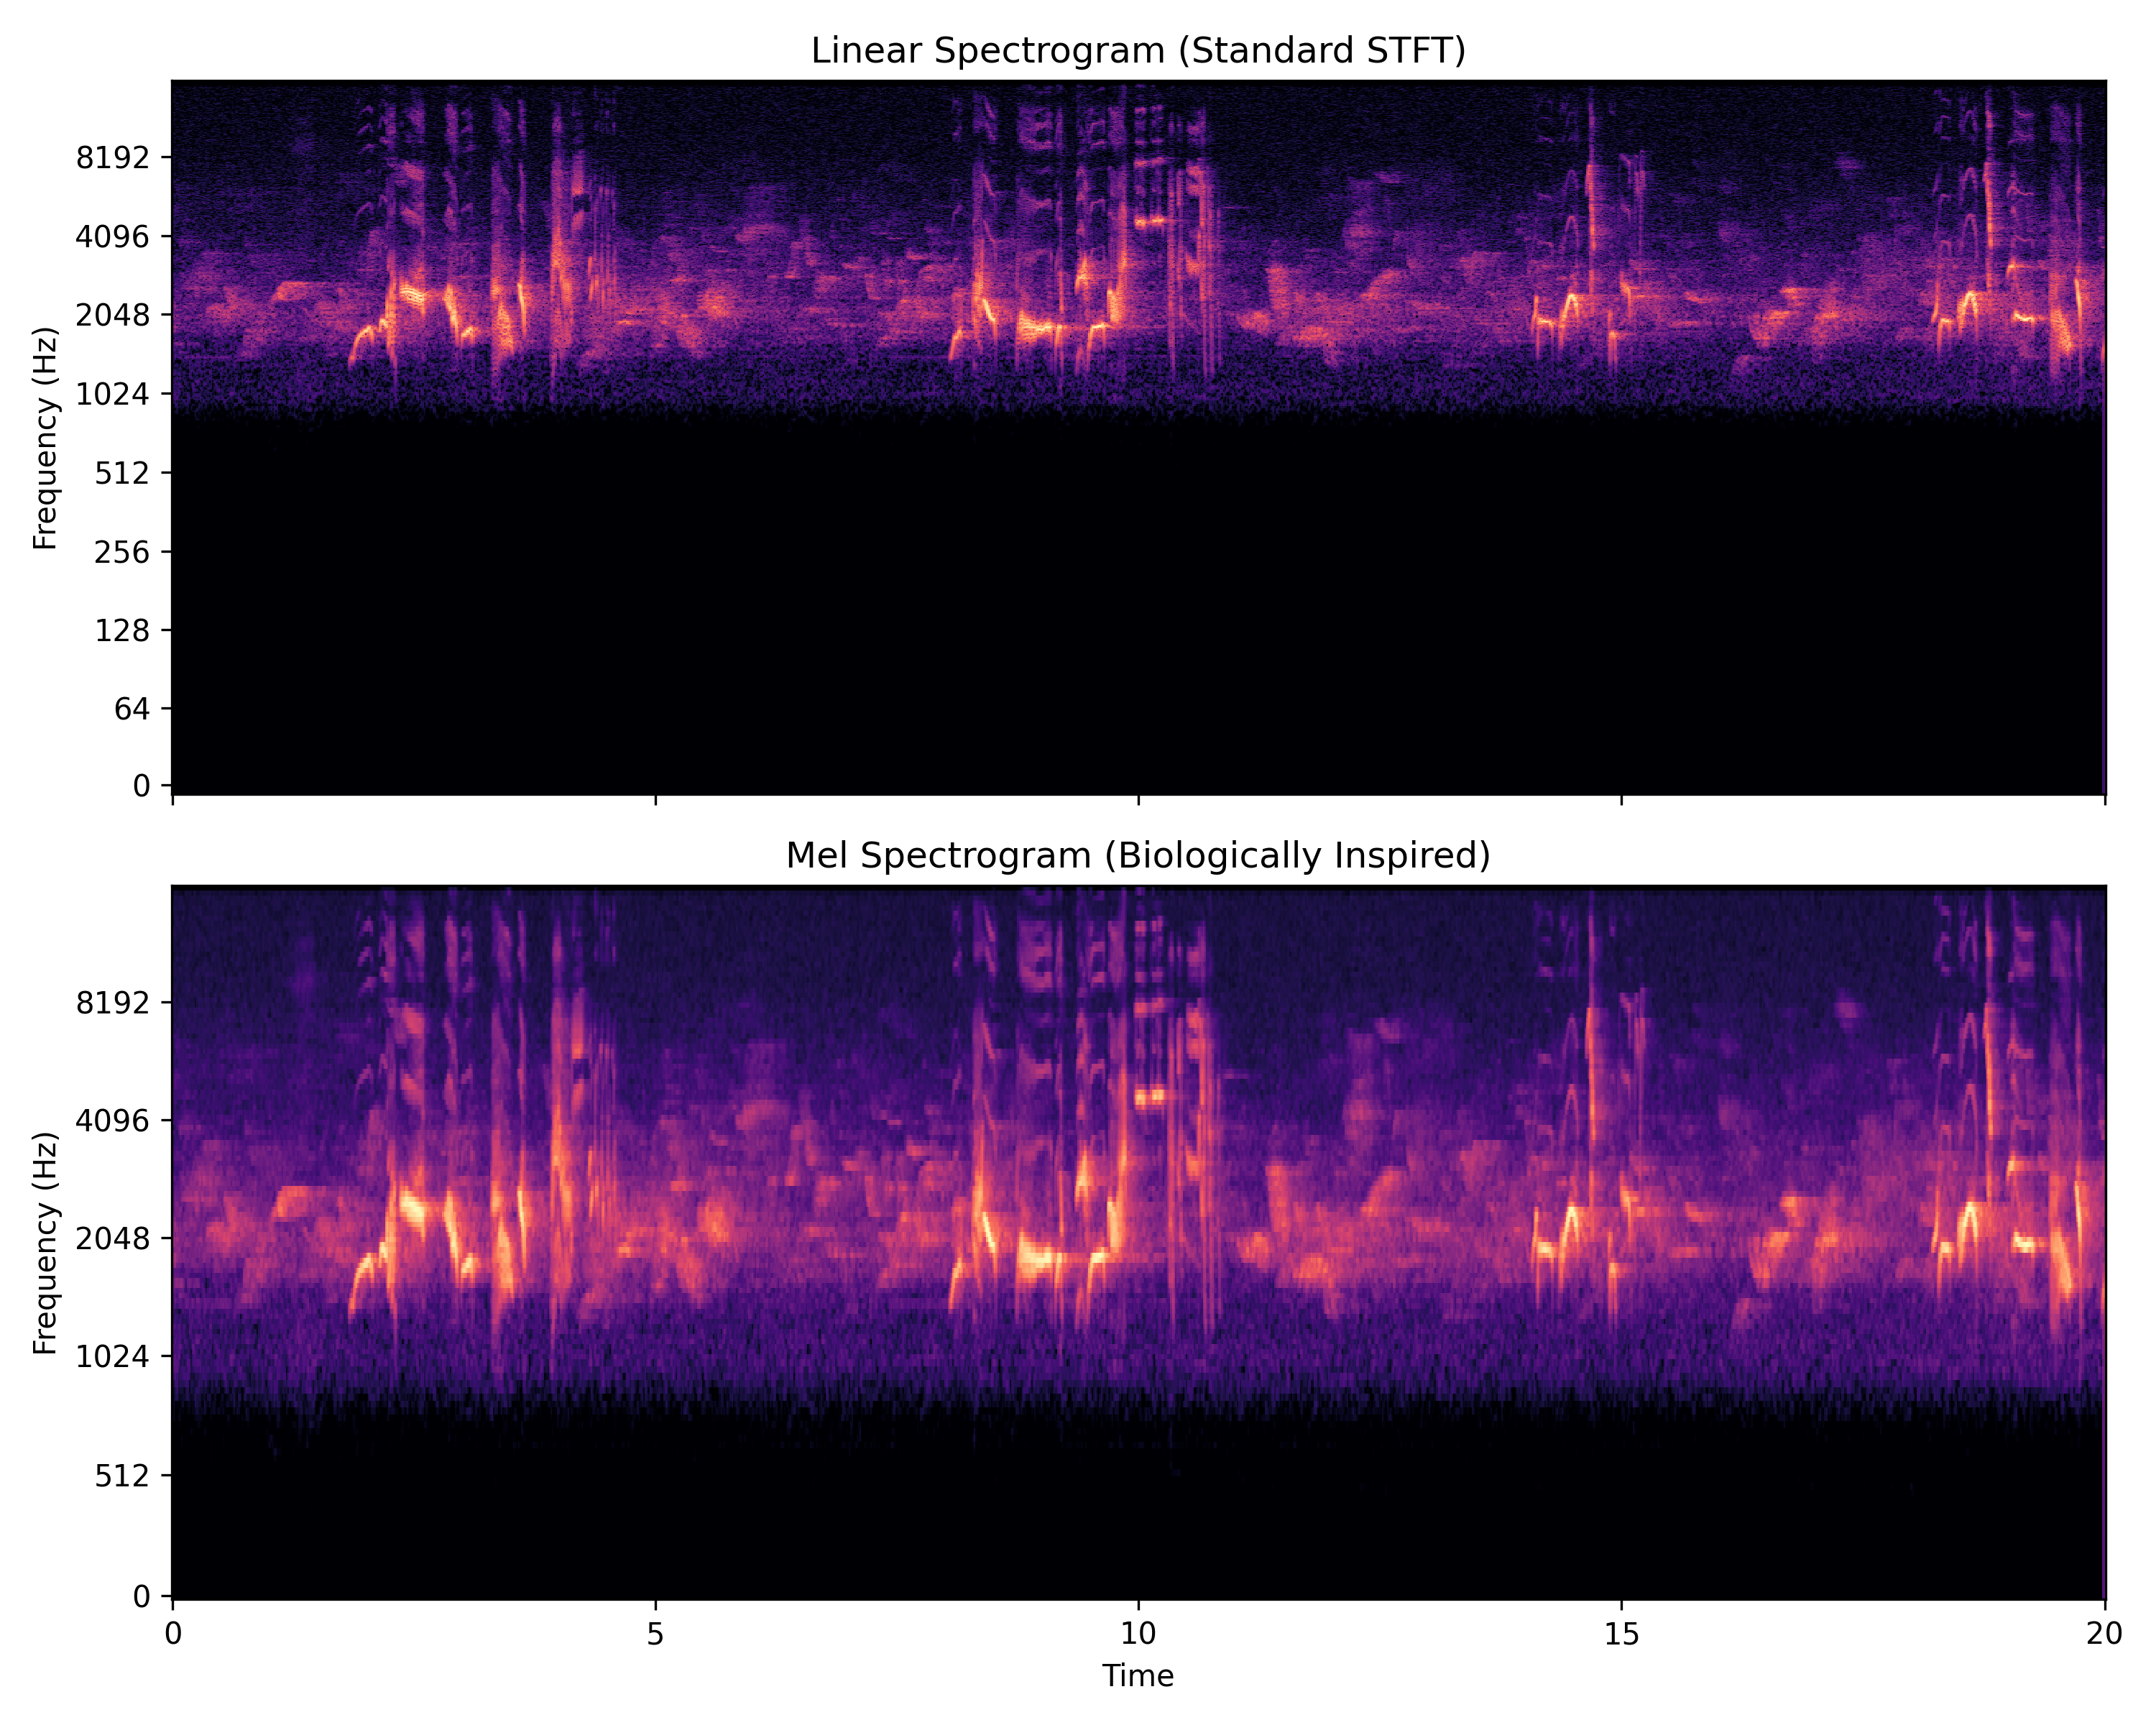
\includegraphics[width=0.75\textwidth]{../visuals/experiments/comparison_linear_vs_mel.png}
    \caption{Vergleich: Das Mel-Spektrogramm (unten) löst die relevanten Frequenzstrukturen des Vogelgesangs deutlich besser auf als die lineare Darstellung (oben).}
    \label{fig:mel_vs_lin}
\end{figure}

\subsection{Artenvielfalt im Bild}
Es ist faszinierend zu sehen, wie unterschiedlich die Arten bereits visuell sind. Eine Amsel sieht im Spektrogramm ganz anders aus als ein Haussperling. Abbildung \ref{fig:species_comp} zeigt exemplarisch fünf zufällig ausgewählte Arten aus unserem Datensatz, um die visuelle Unterscheidbarkeit zu demonstrieren.

\begin{figure}[H]
    \centering
    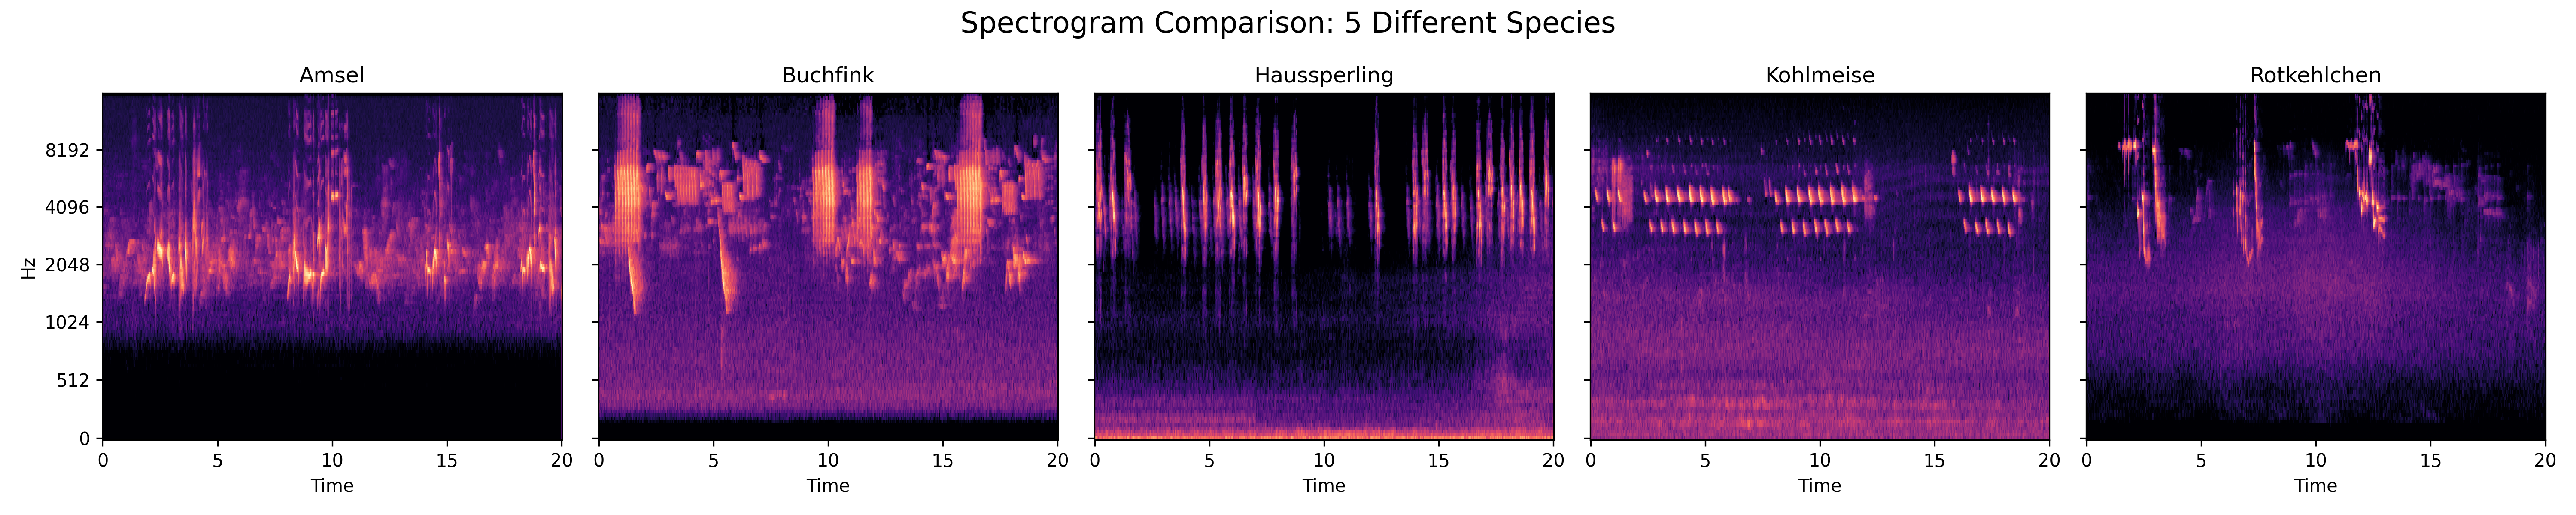
\includegraphics[width=0.85\textwidth]{../visuals/experiments/comparison_species.png}
    \caption{Exemplarische Spektrogramme von fünf Arten aus unserem umfangreichen Europa-Datensatz. Die visuellen Strukturen sind deutlich unterscheidbar, was dem CNN die Klassifikation ermöglicht.}
    \label{fig:species_comp}
\end{figure}

\section{Vorgehensweise und Methoden}

\subsection{Datenpipeline: Der europäische Datensatz}
Die Trainingsdaten stammen aus der Open-Source-Datenbank \textit{Xeno-Canto} \cite{xenocanto}. Unser Skript extrahiert gezielt Aufnahmen aus der Region Europa. Um das Modell für den realen Feldeinsatz zu härten, wurden neben Studioaufnahmen (Qualität A) bewusst auch verrauschte Aufnahmen (Qualität B und C) in den Datensatz integriert. Die Pipeline verarbeitet die Audiodaten direkt: Resampling auf 32\,kHz, Segmentierung in 5-Sekunden-Abschnitte, Transformation in Mel-Spektrogramme (128 Frequenzbänder) und logarithmische Normalisierung (dB) auf Werte zwischen 0 und 1.

\subsection{Modellarchitektur und Trainingstiefe}
Um die enorm hohe Klassenanzahl europäischer Vögel auf ressourcenbeschränkter Edge-Hardware (Raspberry Pi) klassifizieren zu können, fiel unsere Wahl auf die \textbf{EfficientNet-B0} Architektur \cite{tan2019}.
\begin{itemize}
	\item \textbf{Transfer Learning:} Das Netz wurde mit ImageNet-Gewichten initialisiert. Die bereits erlernten Fähigkeiten zur Kanten- und Texturerkennung beschleunigen das Training auf Spektrogrammen enorm.
    \item \textbf{Metric Learning Ansatz (Alternative):} Parallel testeten wir eine Architektur mit \textit{ArcFace Loss}. Hierbei lernt das Modell hochdimensionale Embeddings, bei denen Gesänge derselben Art im Vektorraum maximiert gebündelt werden. Dies bietet Vorteile bei der Entdeckung gänzlich unbekannter Arten.
\end{itemize}

\subsection{Trainingsstrategie und Regularisierung}
Das Training eines derart großen Modells bringt die Gefahr des \textit{Overfittings} mit sich. Wir trainierten in PyTorch \cite{pytorch} mit dem \textbf{AdamW-Optimizer} und einem \textbf{Cosine-Annealing} Learning-Rate-Scheduler für eine cosinus-förmige Konvergenz der lr gegen 0, dh. die learning rate wird immer kleiner. Zwei Maßnahmen waren für den Erfolg kritisch:
1. \textbf{Klassen-Balance:} Da einige Arten $5000$ Aufnahmen besitzen, andere nur $50$, implementierten wir einen \textit{WeightedRandomSampler}. Er sorgt dafür, dass das Netz in jeder Epoche seltene Vögel künstlich öfter zu sehen bekommt.
2. \textbf{SpecAugment:} Während des Trainings werden zufällige Frequenzbänder und Zeitabschnitte im Spektrogramm maskiert. Das Netz wird gezwungen, redundante Merkmale zu lernen und Vögel selbst bei teilweiser Überlagerung durch Windgeräusche zu erkennen. Dies erklärt auch den Verlauf unserer Fehlerkurve (Abbildung \ref{fig:loss_curve}), bei der der Validierungsfehler zeitweise sogar unter dem Trainingsfehler liegt.

\begin{figure}[H]
    \centering
    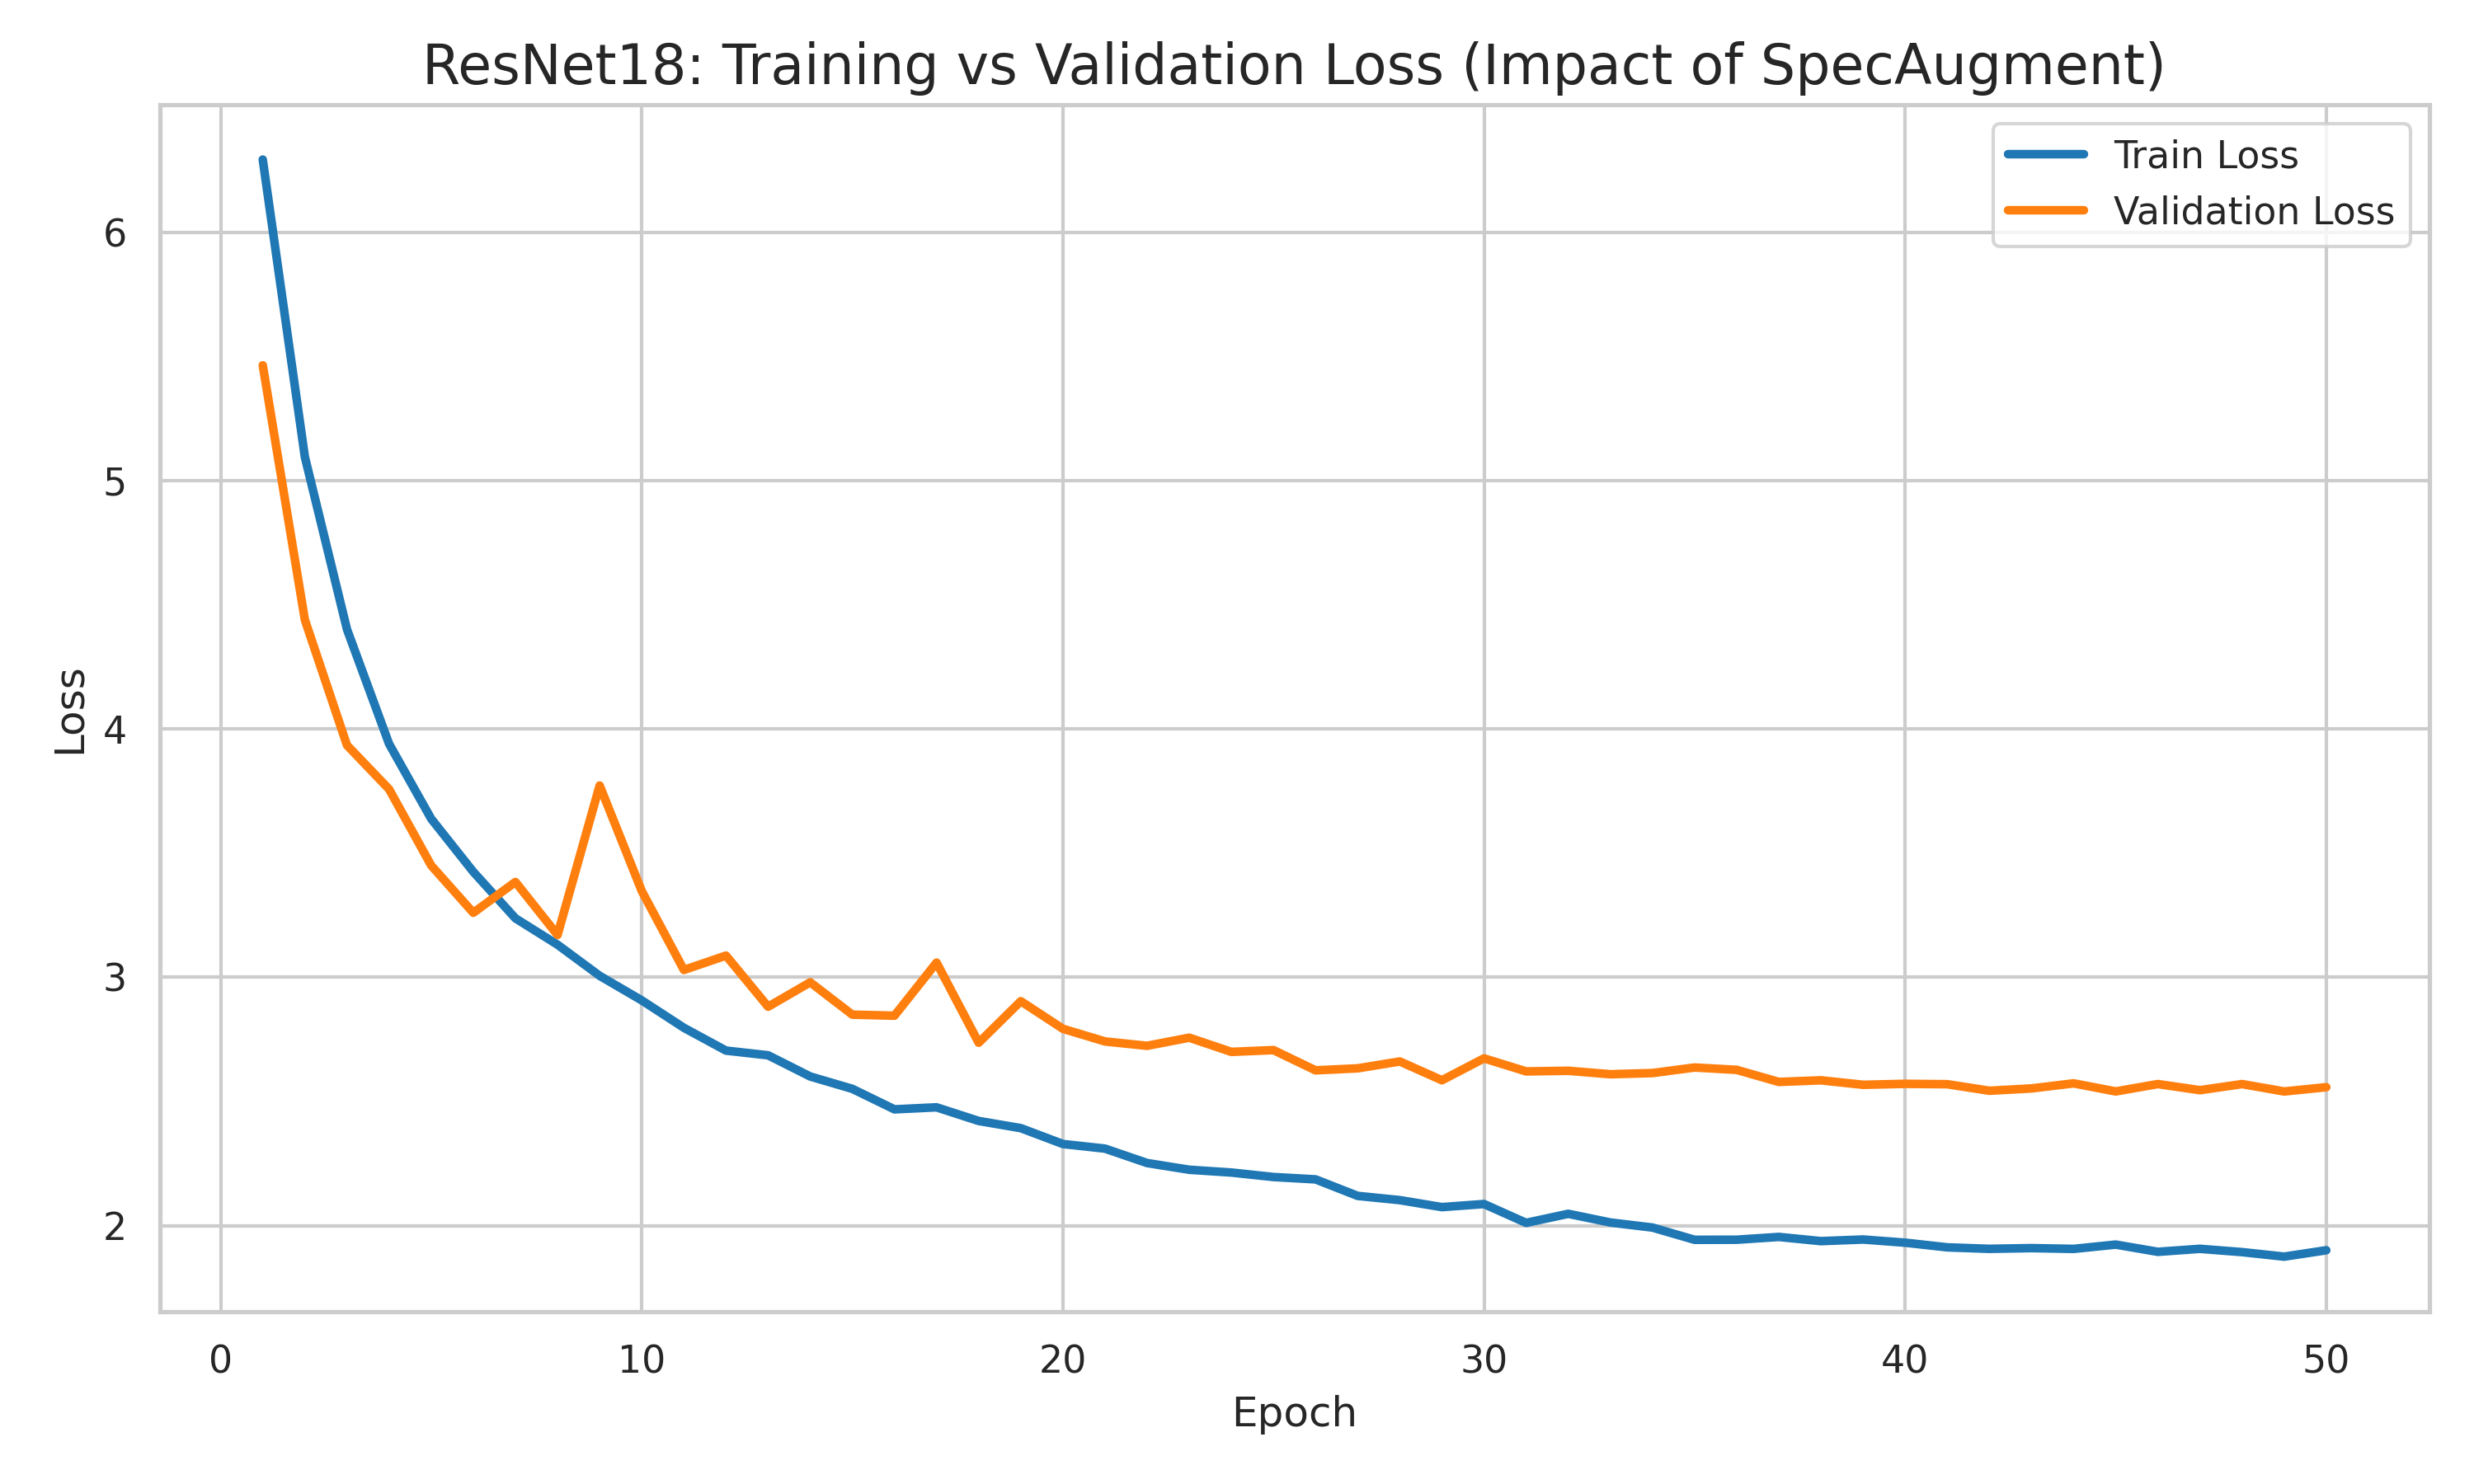
\includegraphics[width=0.65\textwidth]{../visuals/experiments/europe/loss_curve_15epoch_resnet18pre.png}
    \caption{Trainingsverlauf: Normalerweise ist es ein Anzeichen von Overfitting, wenn der Val-Loss deutlich höher als der Train-Loss ist. Bei uns ist der Grund hierfür jedoch, dass wir im Training gezielt Rauschen (SpecAugment) hinzufügen, um das Modell robuster zu machen.}
    \label{fig:loss_curve}
\end{figure}

\section{Ergebnisse und Evaluation}

\subsection{Trefferquote und Datenabhängigkeit}
Unser Transfer-Learning-Ansatz (EfficientNet) erzielte auf den Validierungsdaten exzellente Ergebnisse und dominierte unsere klassischen \enquote{From-Scratch} trainierte Custom-CNNs deutlich, selbst mit Attention können unsere Custom CNNs nicht mithalten. (Abb. \ref{fig:performance_group}a). Abbildung \ref{fig:performance_group}b zeigt zudem erwartungsgemäß, dass Arten mit einem größeren Datenvolumen (große Blasen) eine höhere Klassifikationssicherheit aufweisen, weshalb das Sammeln weiterer Felddaten ein fortlaufender Prozess bleibt.

\begin{figure}[H]
    \centering
    \begin{subfigure}[b]{0.48\textwidth}
        \centering
        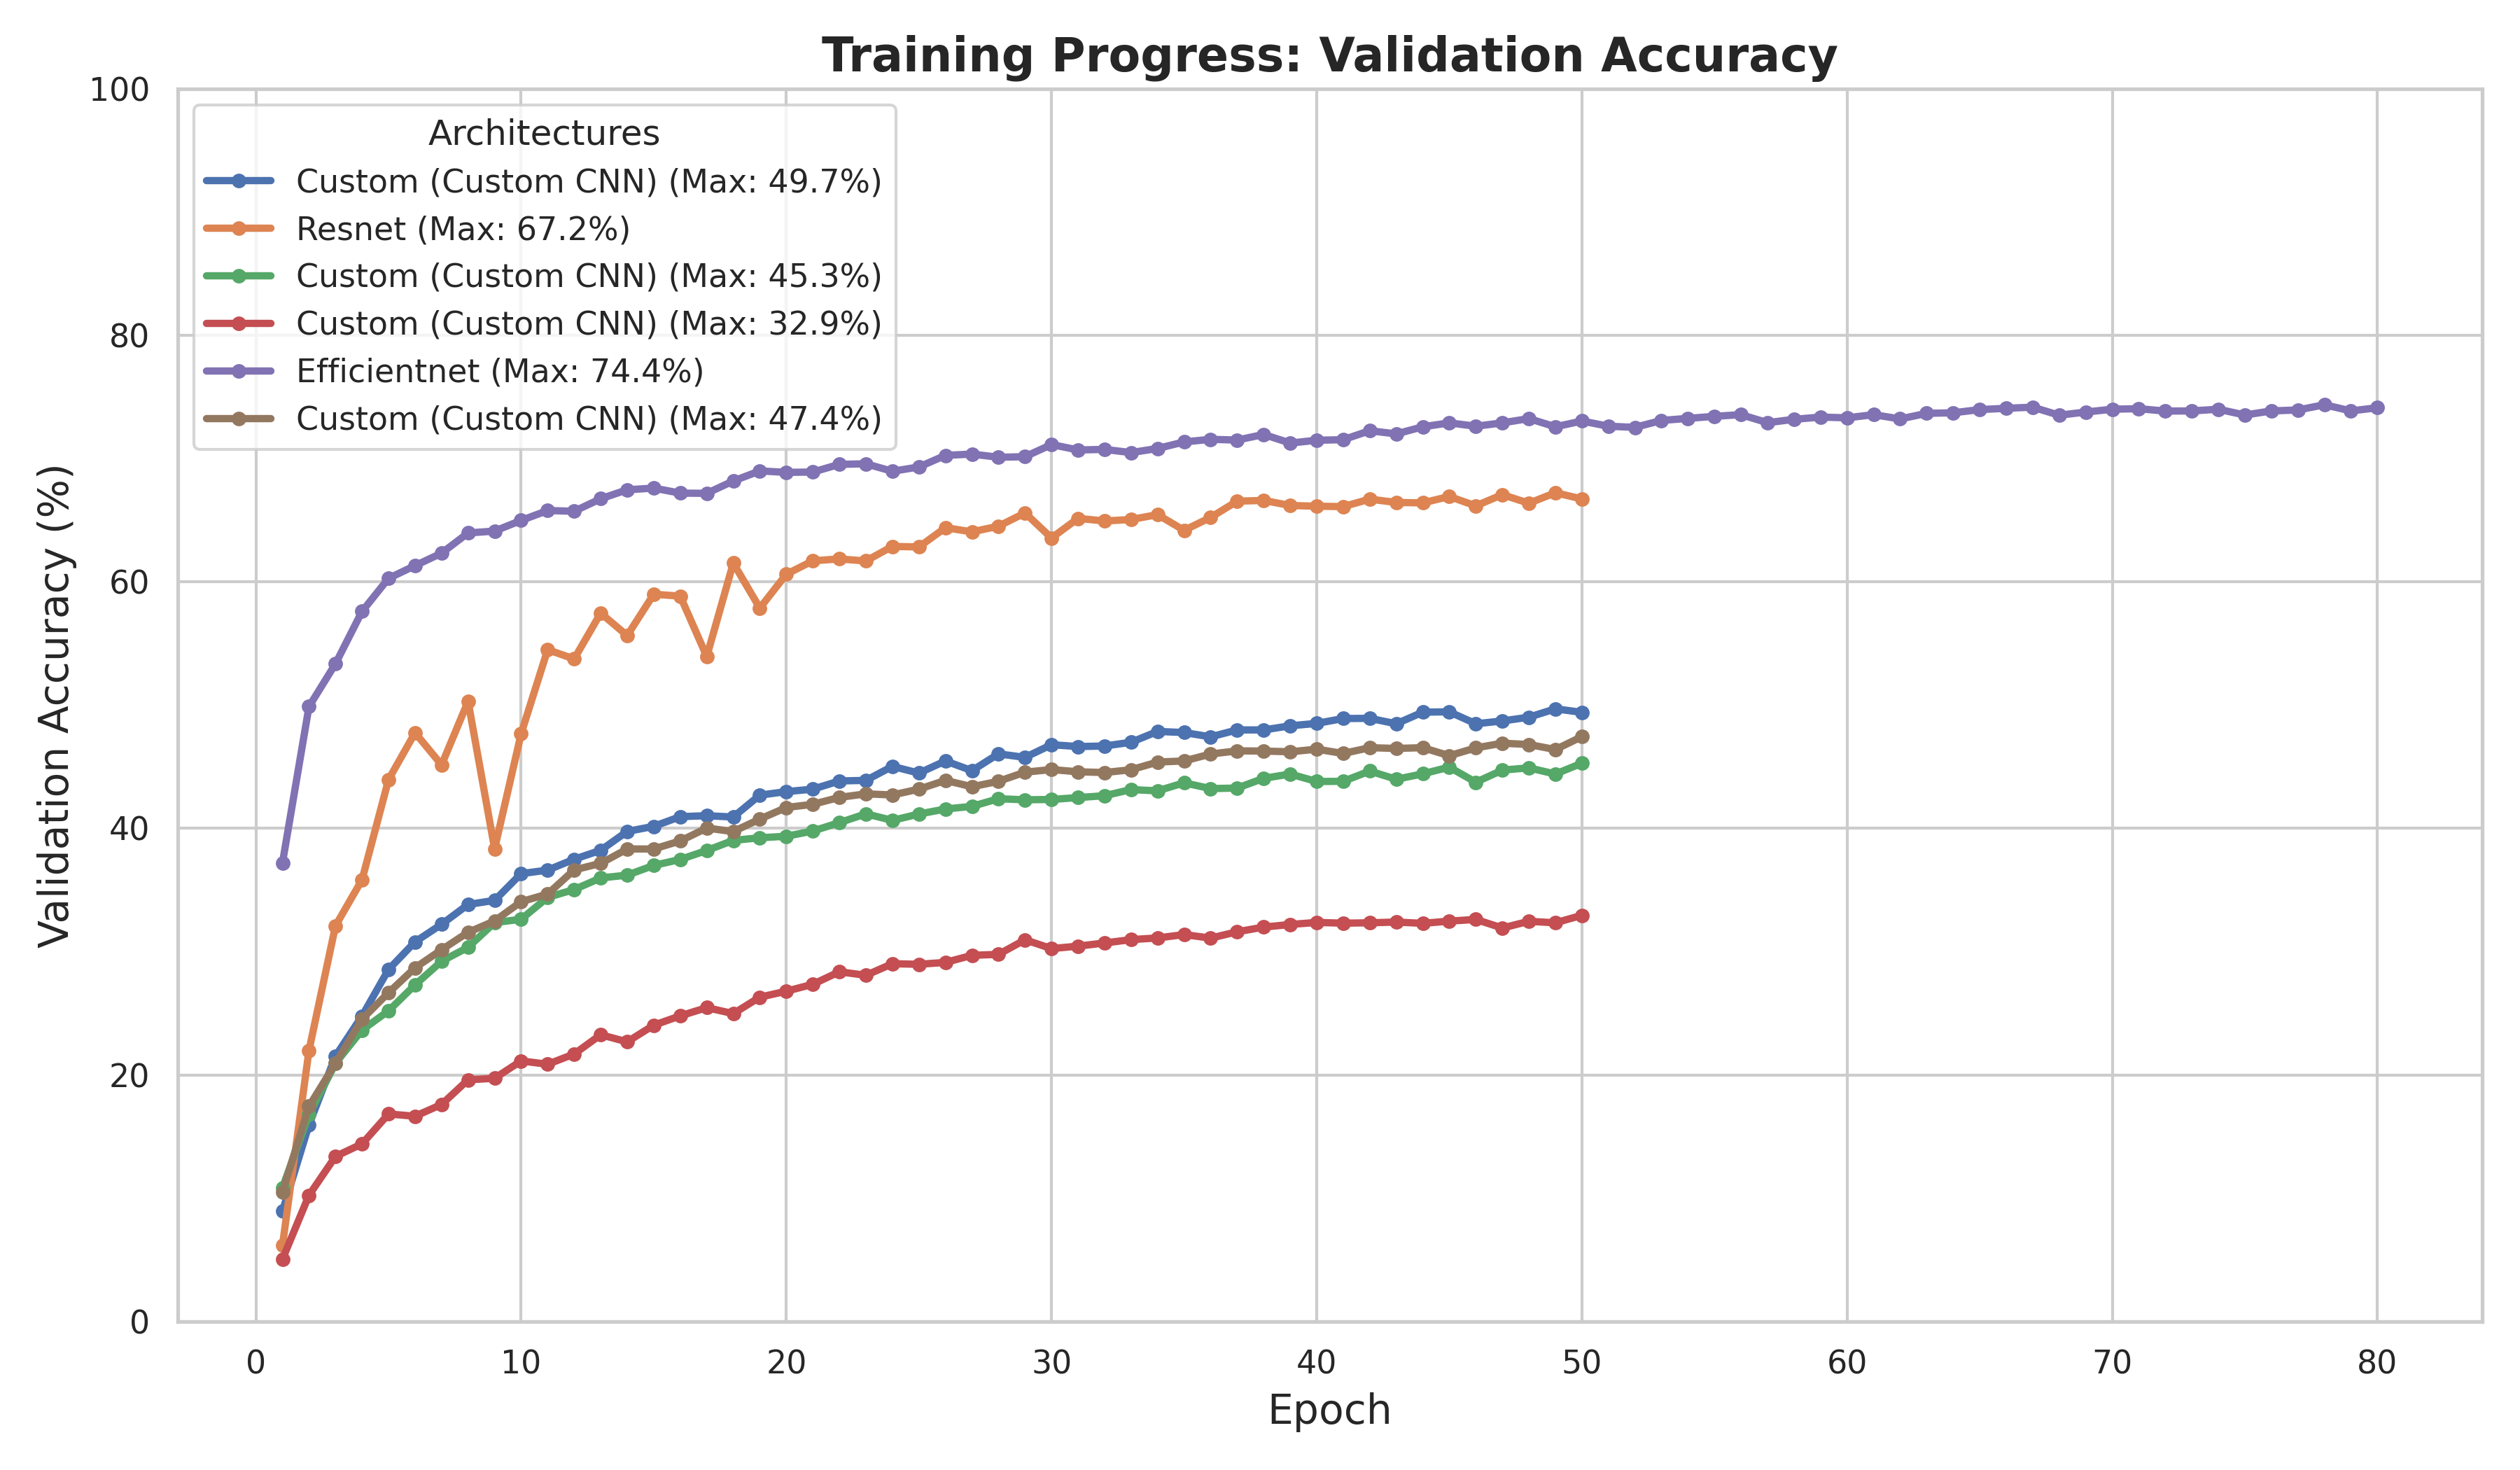
\includegraphics[width=\textwidth]{../visuals/experiments/europe/comparison_model_performance.png}
        \caption{Das Transfer-Learning-Modell (EfficientNet) dominiert deutlich und generalisiert am besten.}
    \end{subfigure}
    \hfill
    \begin{subfigure}[b]{0.48\textwidth}
        \centering
        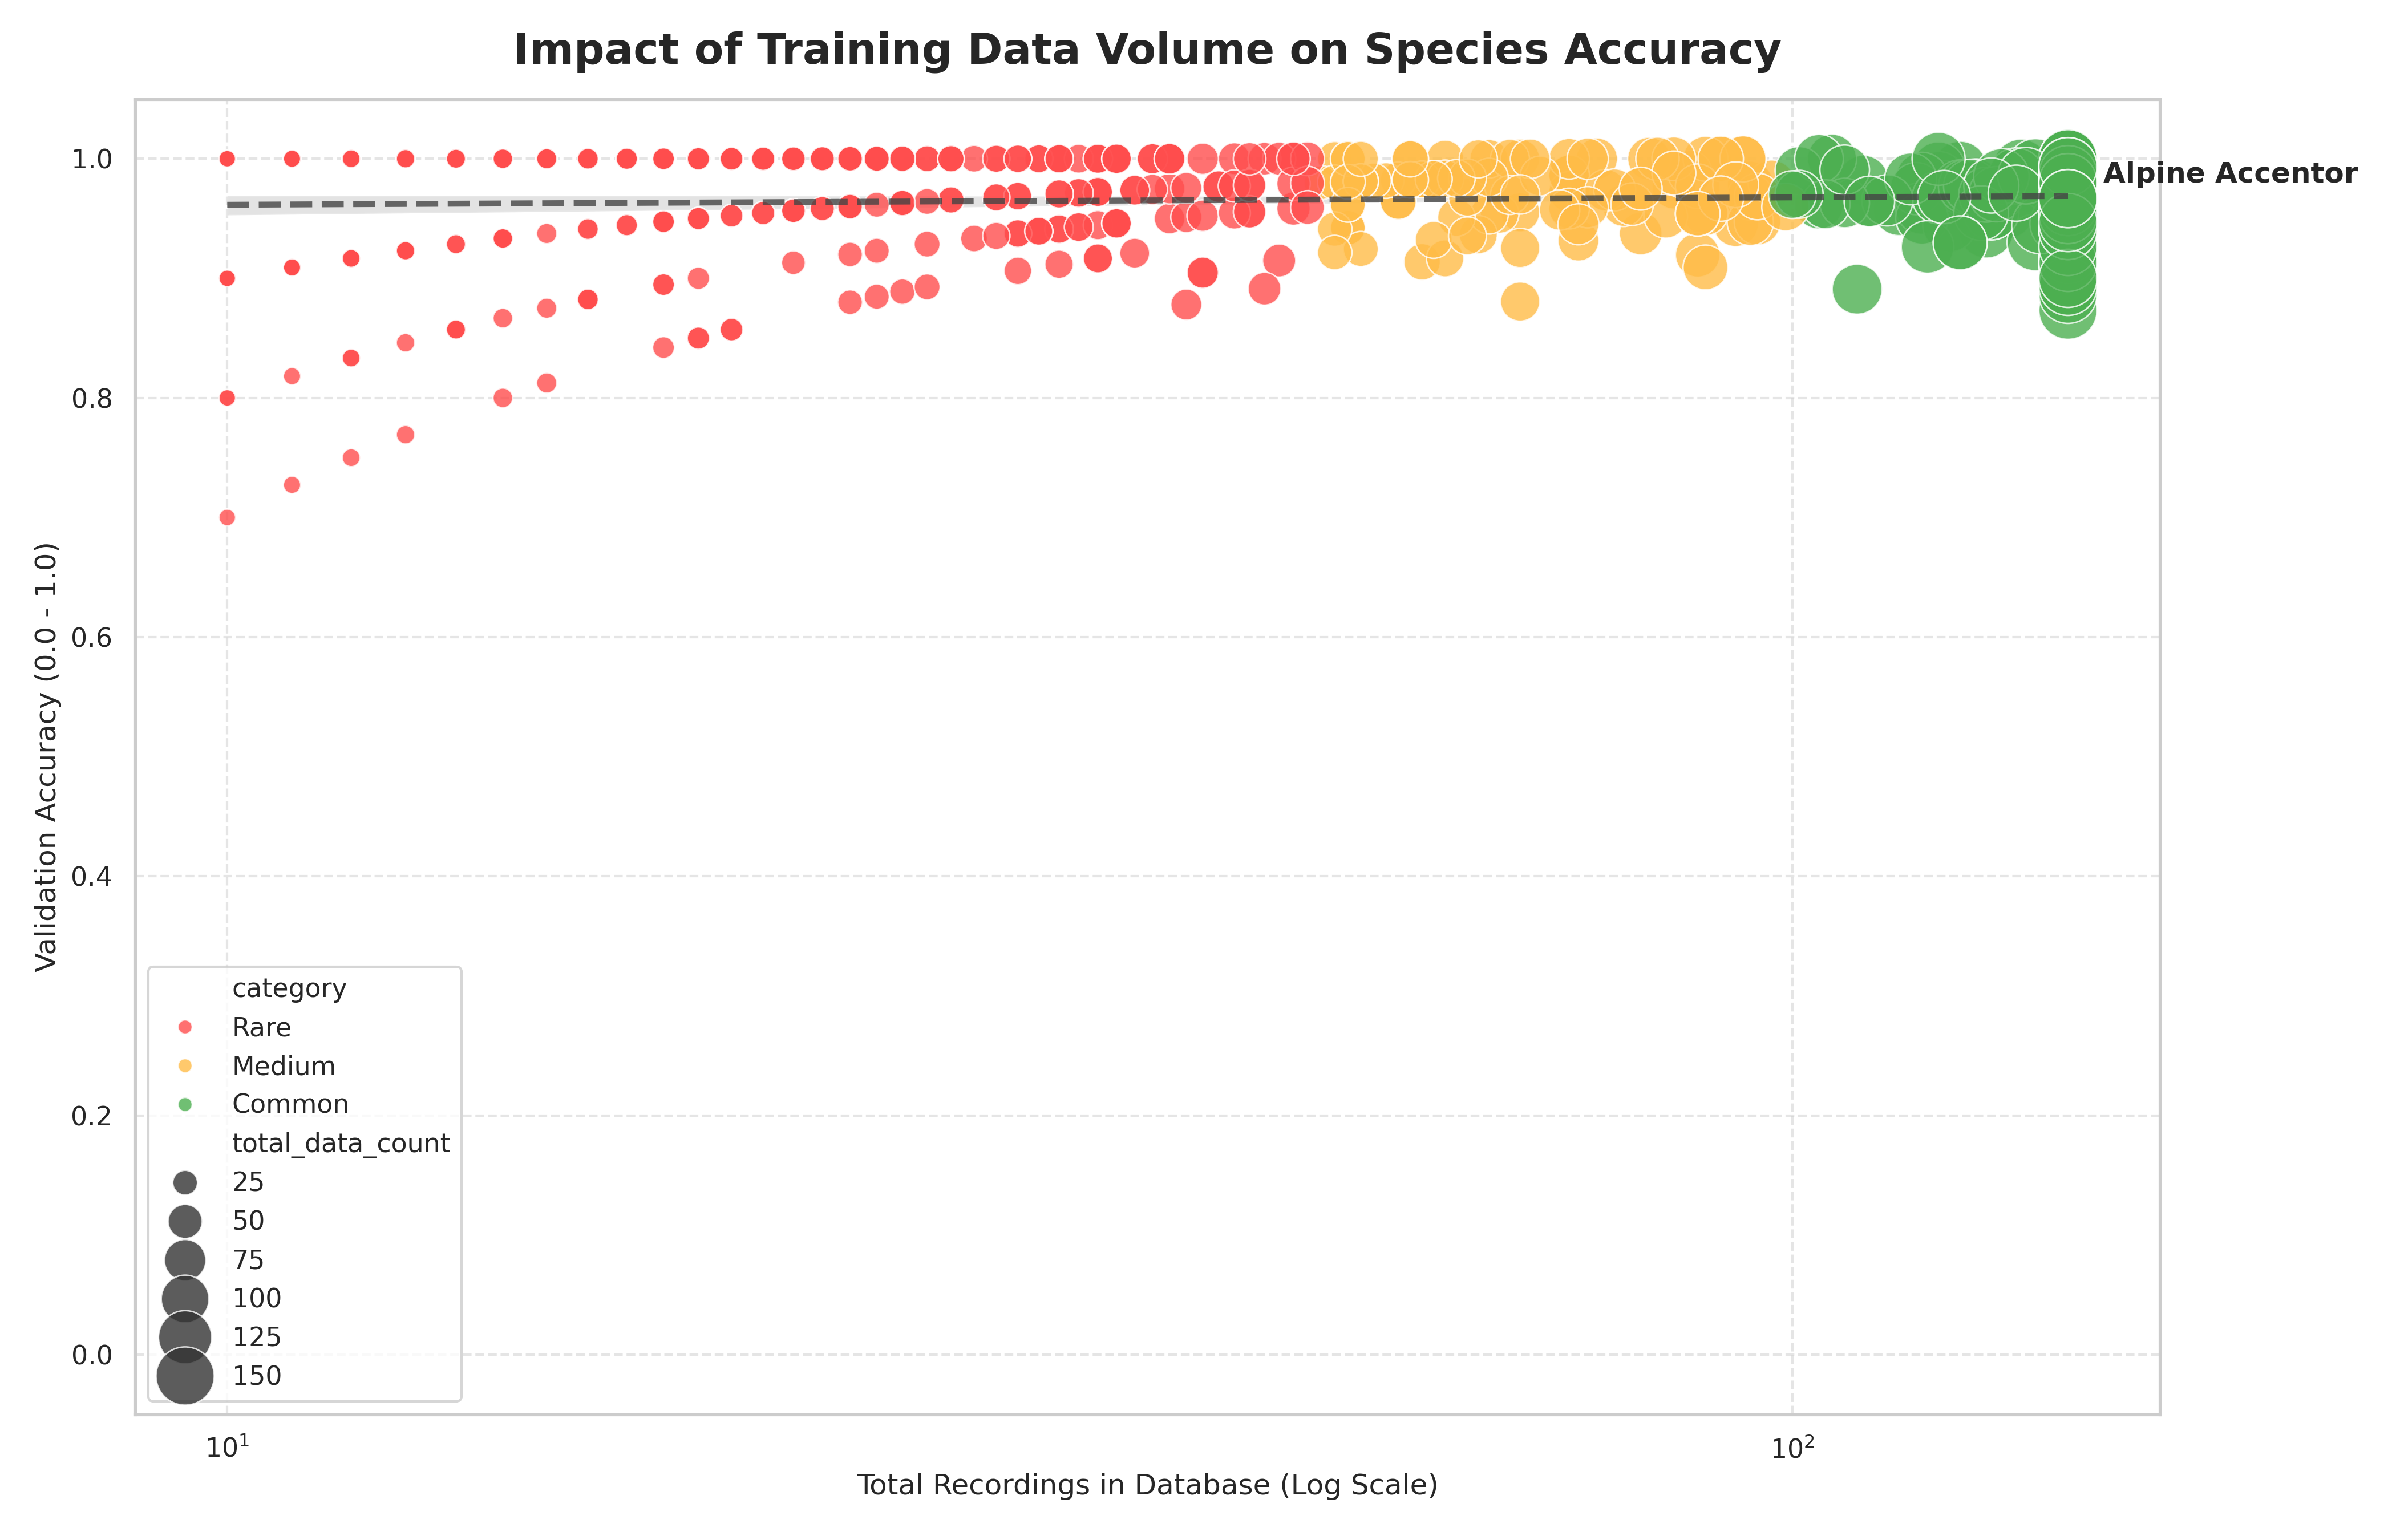
\includegraphics[width=\textwidth]{../visuals/experiments/europe/scatter_data_vs_acc_bubble.png}
        \caption{Einfluss der Datenmenge auf die Genauigkeit (Blasengröße = Datensatzgröße).}
    \end{subfigure}
    \caption{Modellvergleich und Datenabhängigkeit.}
    \label{fig:performance_group}
\end{figure}

\subsection{Fehleranalyse}
Natürlich ist keine KI perfekt. Wir haben die Fehler genau analysiert. Die Konfusionsmatrix in Abbildung \ref{fig:error_analysis}a zeigt exemplarisch das finale Modell auf den Testdaten. Die Diagonale ist sehr ausgeprägt, was für eine hohe Genauigkeit spricht. In Abbildung \ref{fig:error_analysis}b haben wir die häufigsten Fehlklassifikationen genauer aufgeschlüsselt. Verwechslungen treten vor allem bei sehr kurzen Rufen von verwandten Arten auf (z.B. verschiedene Finken-Arten). Das ist aber auch für menschliche Experten oft schwer zu unterscheiden.

\begin{figure}[H]
    \centering
    \begin{subfigure}[b]{0.48\textwidth}
        \centering
        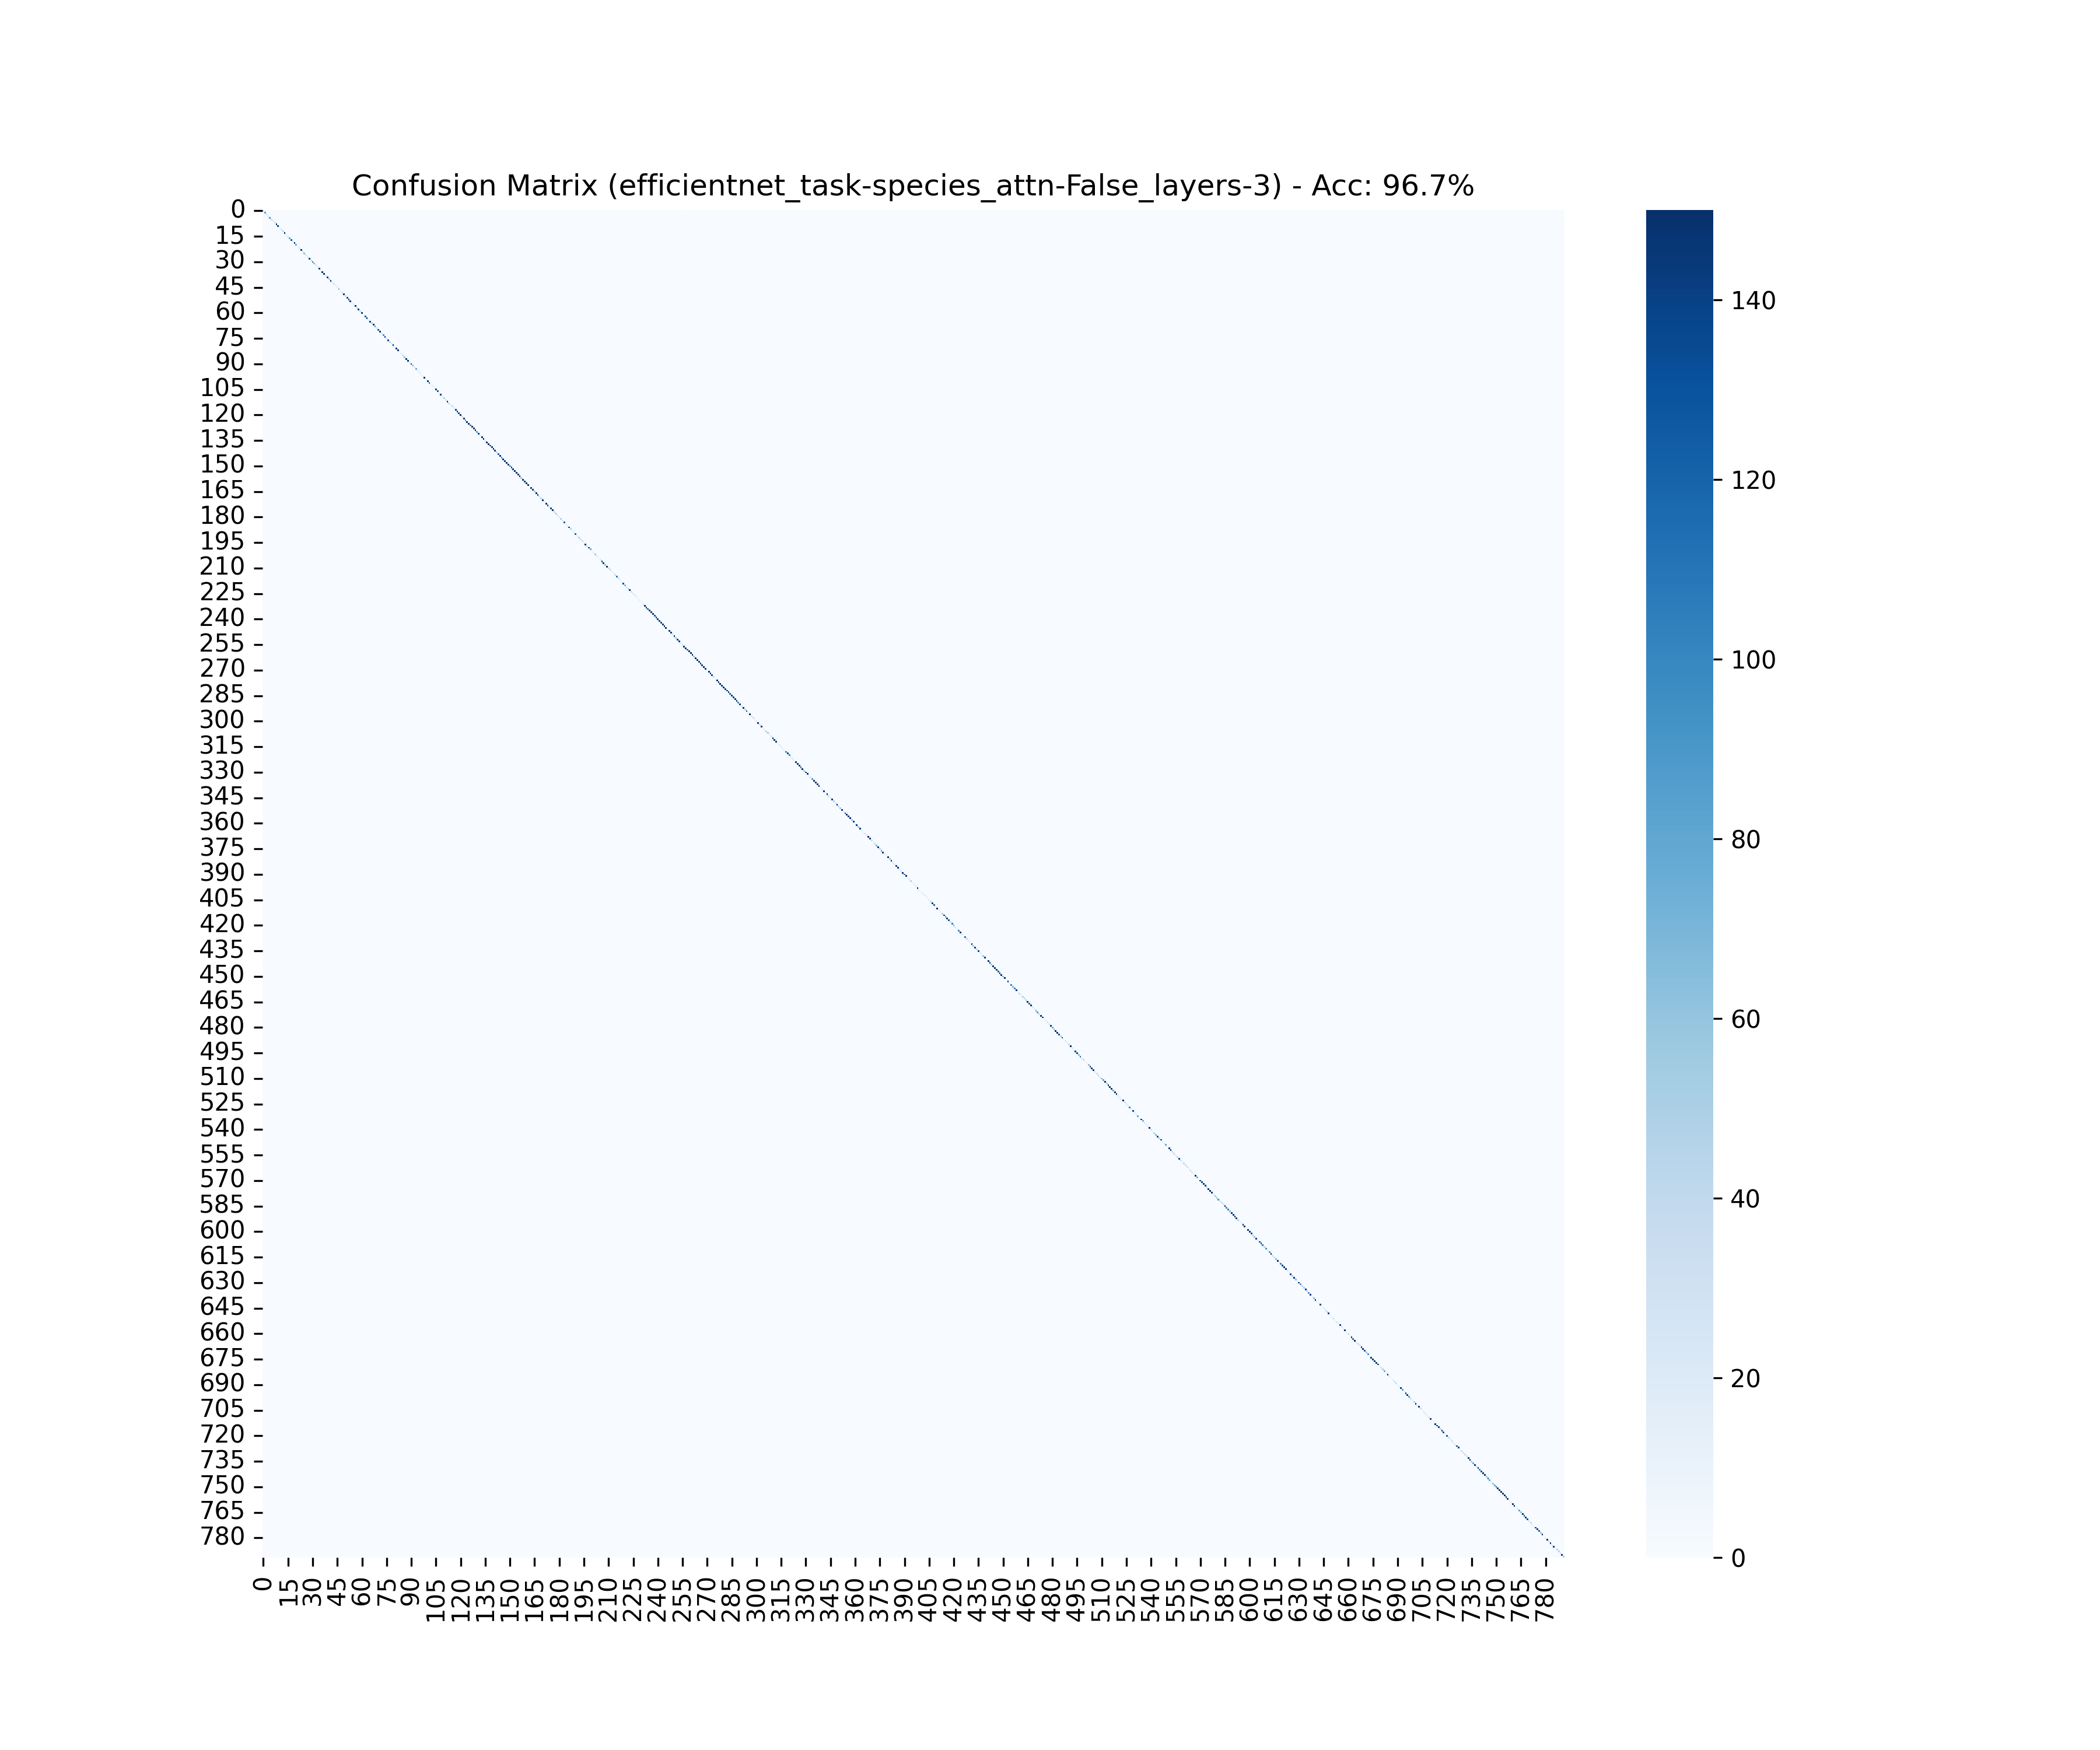
\includegraphics[width=\textwidth]{../visuals/experiments/europe/efficientnet_task-species_attn-False_layers-3_confusion.png}
        \caption{Konfusionsmatrix: Die dichte Diagonale bestätigt die hohe Präzision.}
    \end{subfigure}
    \hfill
    \begin{subfigure}[b]{0.48\textwidth}
        \centering
        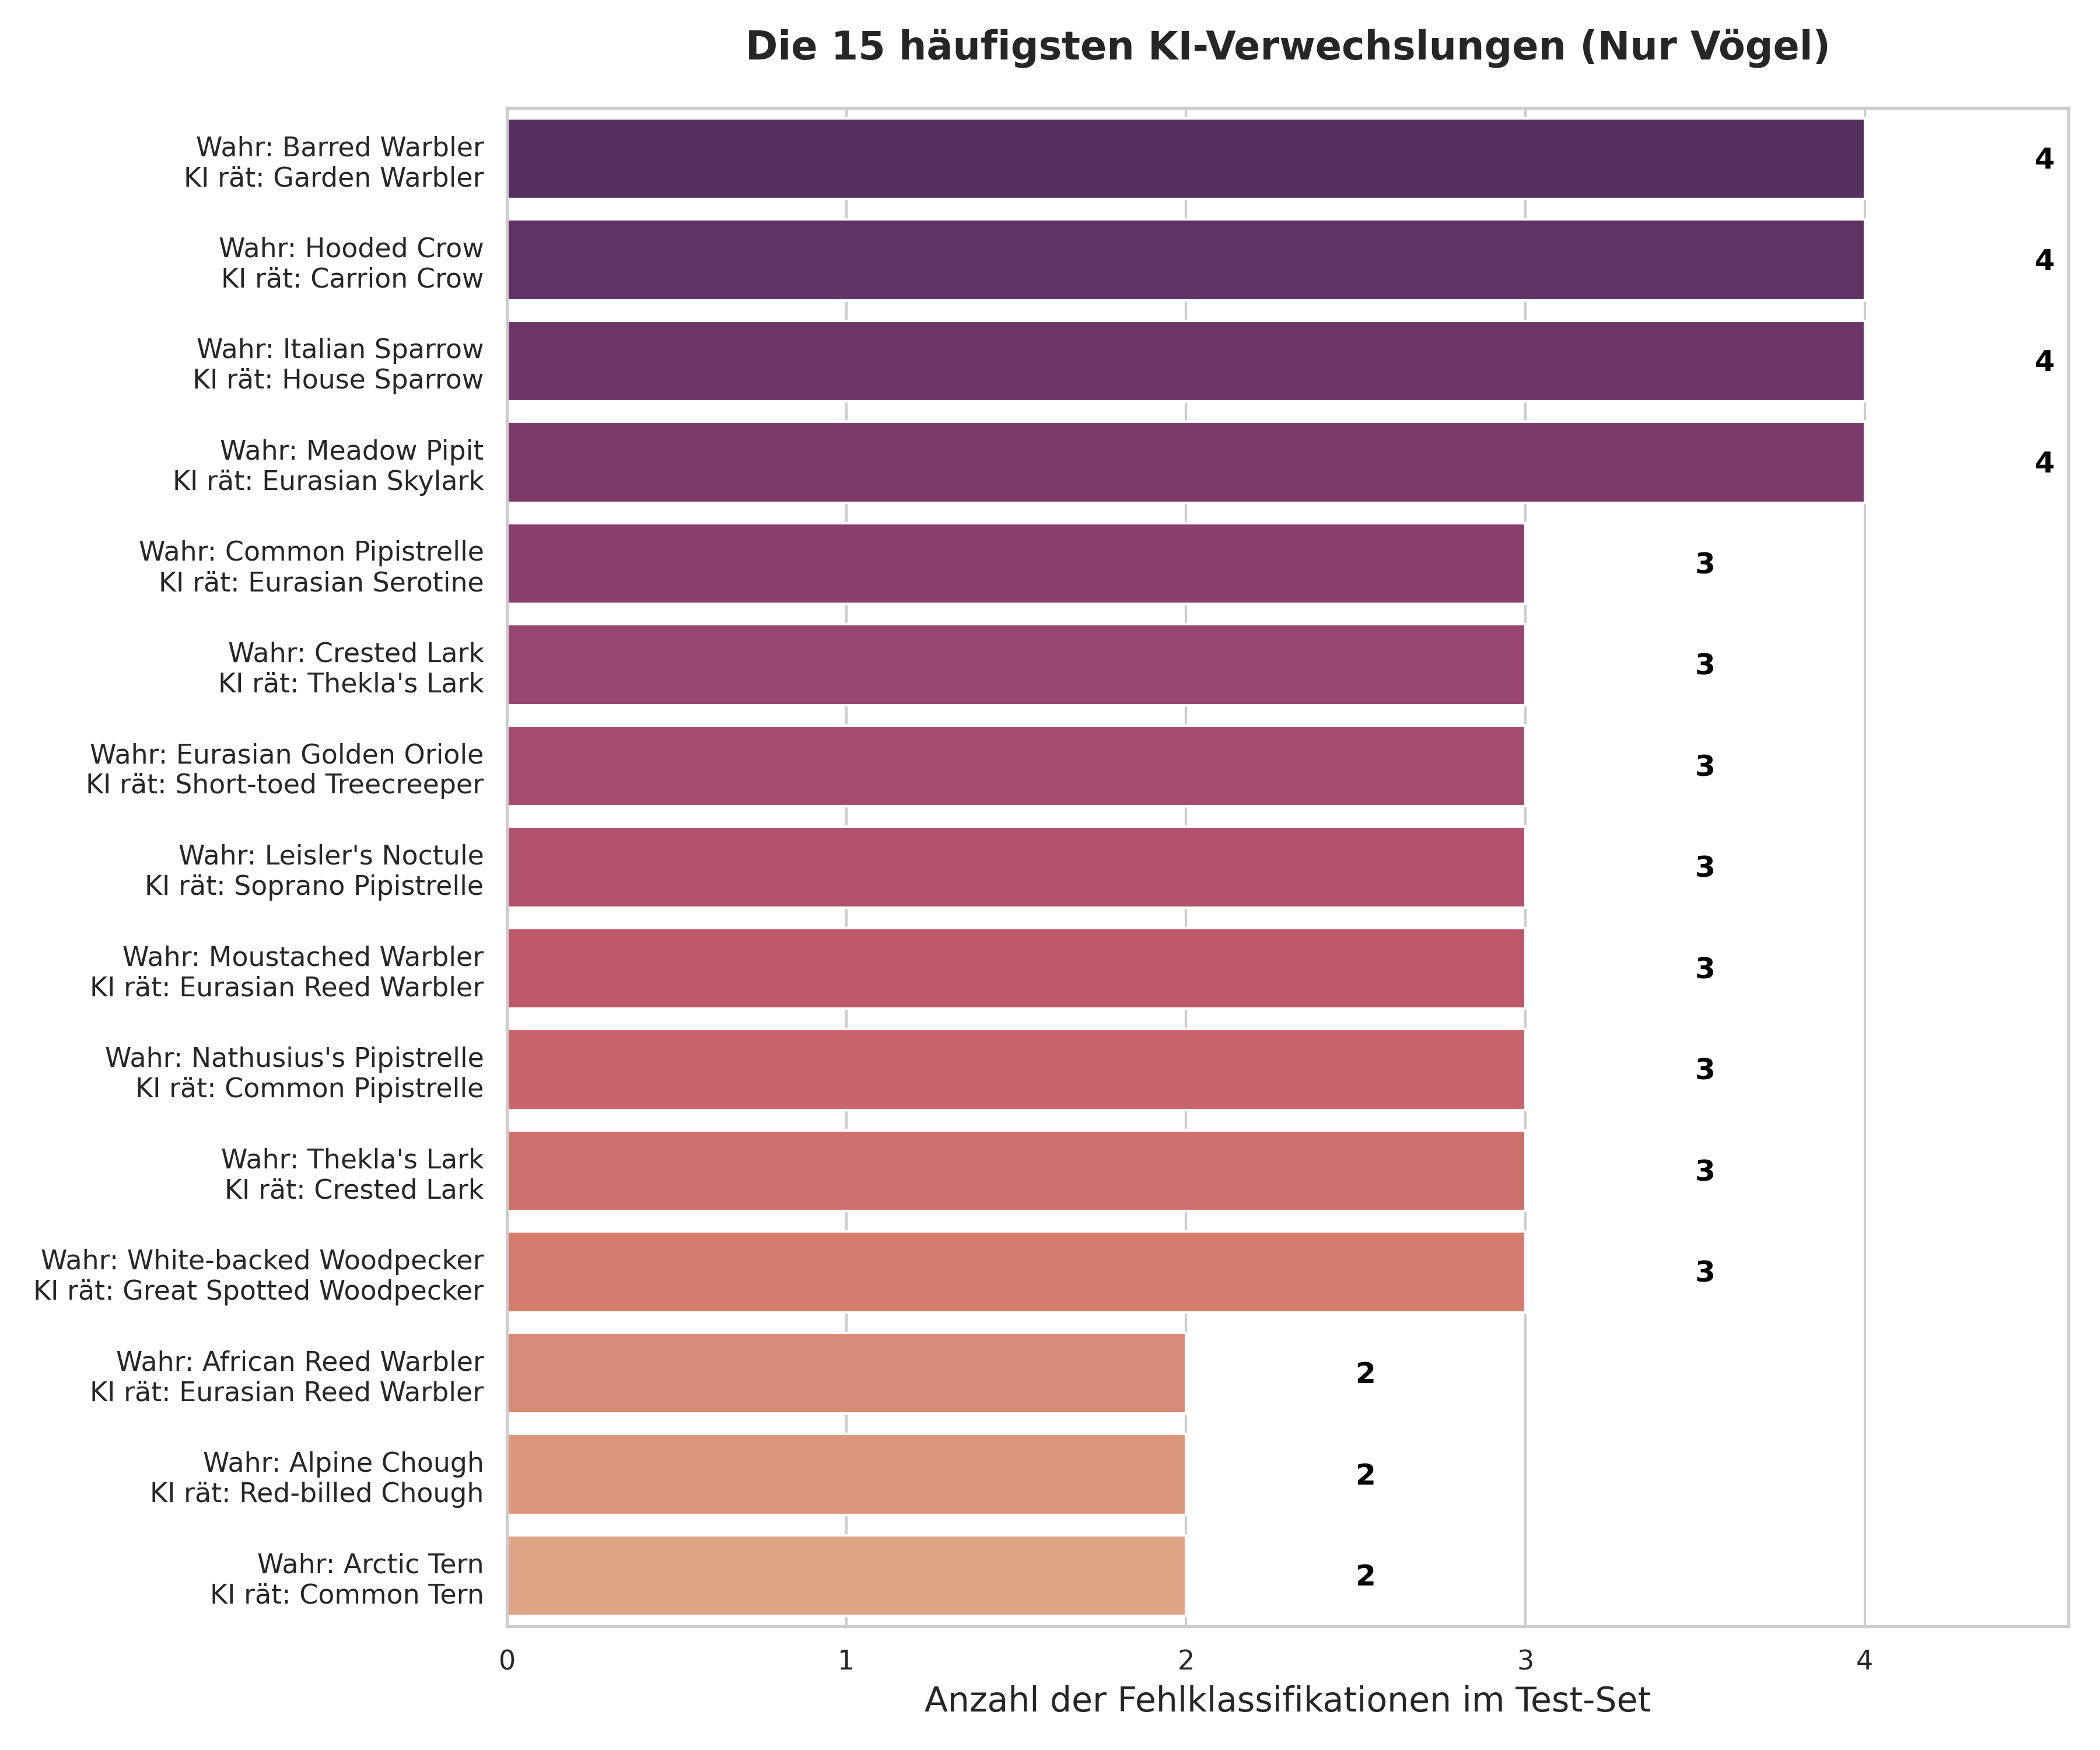
\includegraphics[width=\textwidth]{../visuals/experiments/europe/top_errors.png}
        \caption{Die 15 häufigsten KI-Verwechslungen im Test-Set.}
    \end{subfigure}
    \caption{Fehleranalyse des finalen Modells.}
    \label{fig:error_analysis}
\end{figure}

\subsection{Robustheit gegen schlechte Audioqualität}
Ein wichtiger Punkt war uns die Frage, wie das Modell reagiert, wenn die Aufnahmequalität sinkt. Auf Xeno-Canto sind die Aufnahmen mit Buchstaben von A (Studio) bis E (unbrauchbar) bewertet. In Abbildung \ref{fig:quality} sehen wir, dass die Erkennungsrate bei A-C ungefähr gleichbleibt, unser Modell ist also relativ unabhängig von Audioqualität.

\begin{figure}[H]
    \centering
    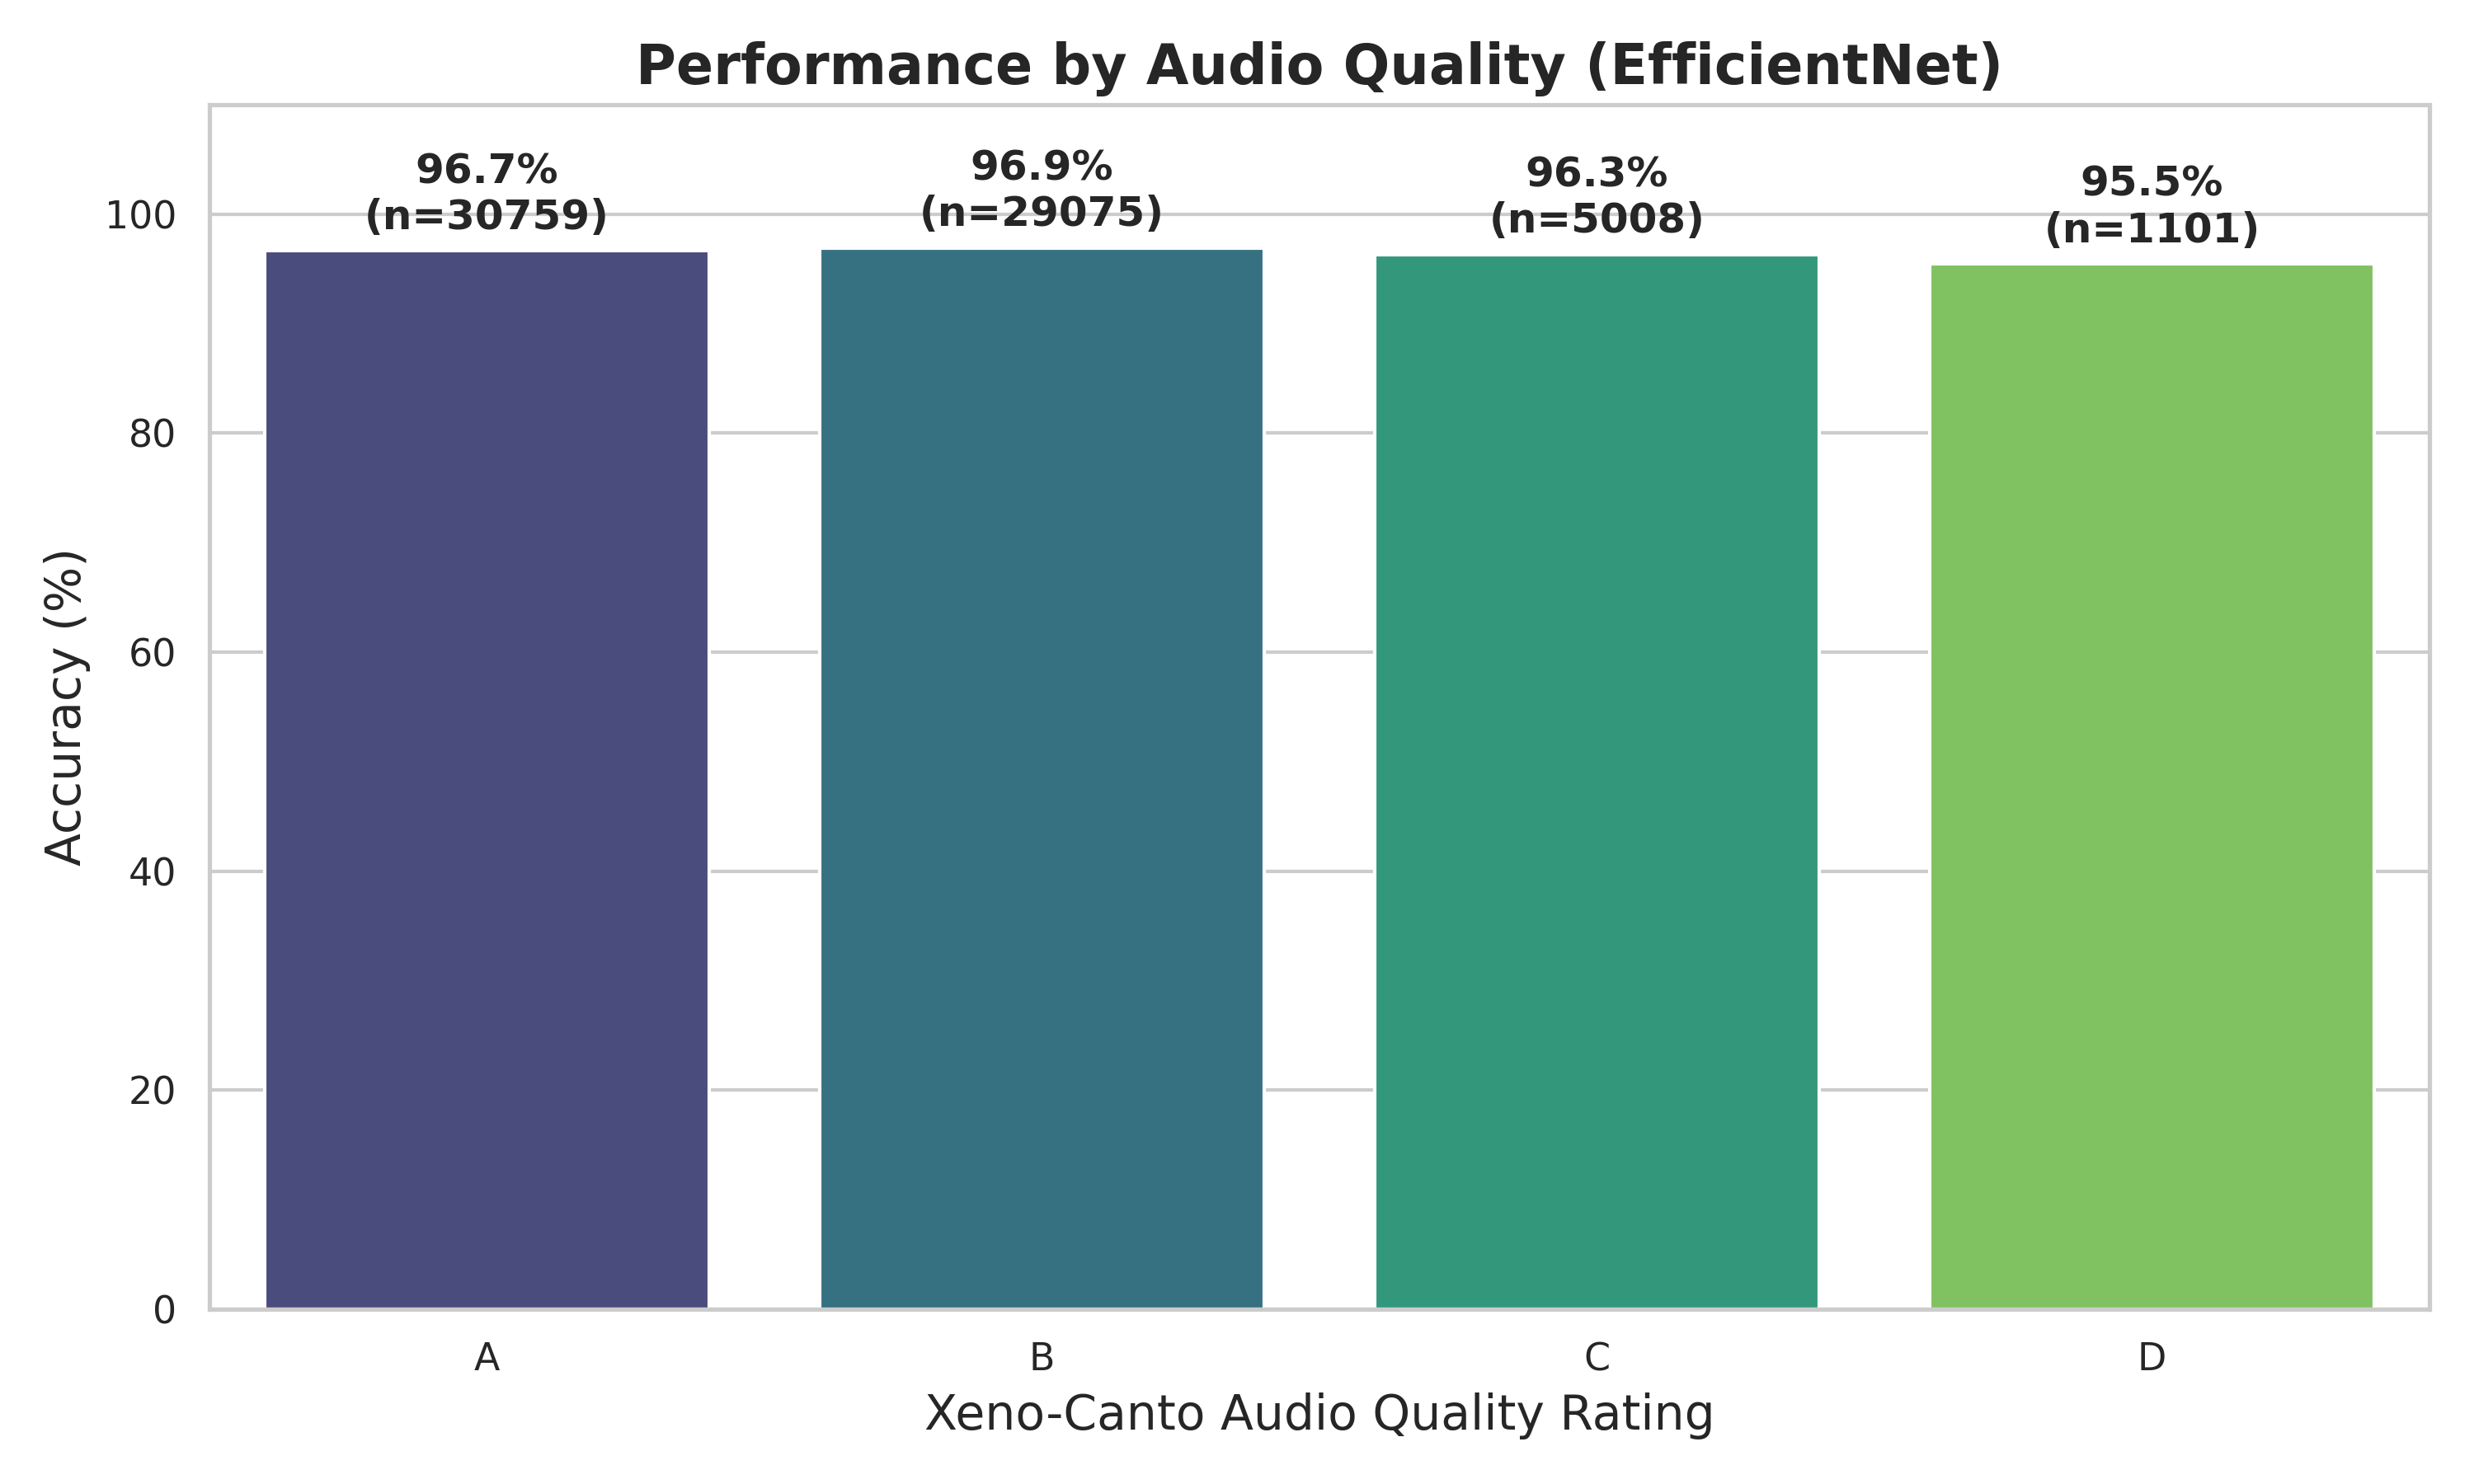
\includegraphics[width=0.6\textwidth]{../visuals/experiments/europe/performance_by_quality.png}
    \caption{Performance nach Audioqualität. Selbst bei schlechten Aufnahmen (D) bleibt das Modell gut nutzbar.}
    \label{fig:quality}
\end{figure}

\subsection{Validierung durch externe Datenquellen (Cross-Testing)}
Ein häufiges Risiko beim Training neuronaler Netze ist der sogenannte \enquote{Dataset Bias} – das Modell lernt dabei nicht nur die Vogelstimmen, sondern versehentlich auch die spezifischen Eigenheiten der Aufnahmegeräte der Trainingsdatenbank. Um sicherzustellen, dass unser Modell generalisiert, haben wir Cross-Tests mit Audioquellen durchgeführt, die nicht Teil des Xeno-Canto-Trainingsdatensatzes waren.

Hierfür nutzten wir exemplarische Aufnahmen aus dem Google AudioSet sowie Referenzaufnahmen der Plattform \textit{kookoo.eu}. Das Modell konnte auch diese artfremden Aufnahmen mit hoher Zuverlässigkeit klassifizieren. Dies bestätigt, dass die KI tatsächlich die spektralen Muster der Vögel gelernt hat und nicht nur auf die akustische Signatur einer spezifischen Datenbank optimiert ist.

\subsection{Zusatzexperimente: Rufe vs. Gesänge und Architekturvergleich}
Neben der Artenerkennung haben wir untersucht, ob das Modell auch den Typ der Lautäußerung (Gesang oder Ruf) unterscheiden kann. Die t-SNE Visualisierung der Embeddings (Abb. \ref{fig:tsne}a) zeigt, dass das Modell diese Unterscheidung intern sehr gut trennt. Zusätzlich haben wir unsere verschiedenen Modellarchitekturen direkt verglichen (siehe Abb. \ref{fig:tsne}b), um den besten Kompromiss aus Parametergröße und Leistungsfähigkeit für das spätere Raspberry Pi Deployment zu ermitteln.

\begin{figure}[H]
    \centering
    \begin{subfigure}[b]{0.45\textwidth}
        \centering
        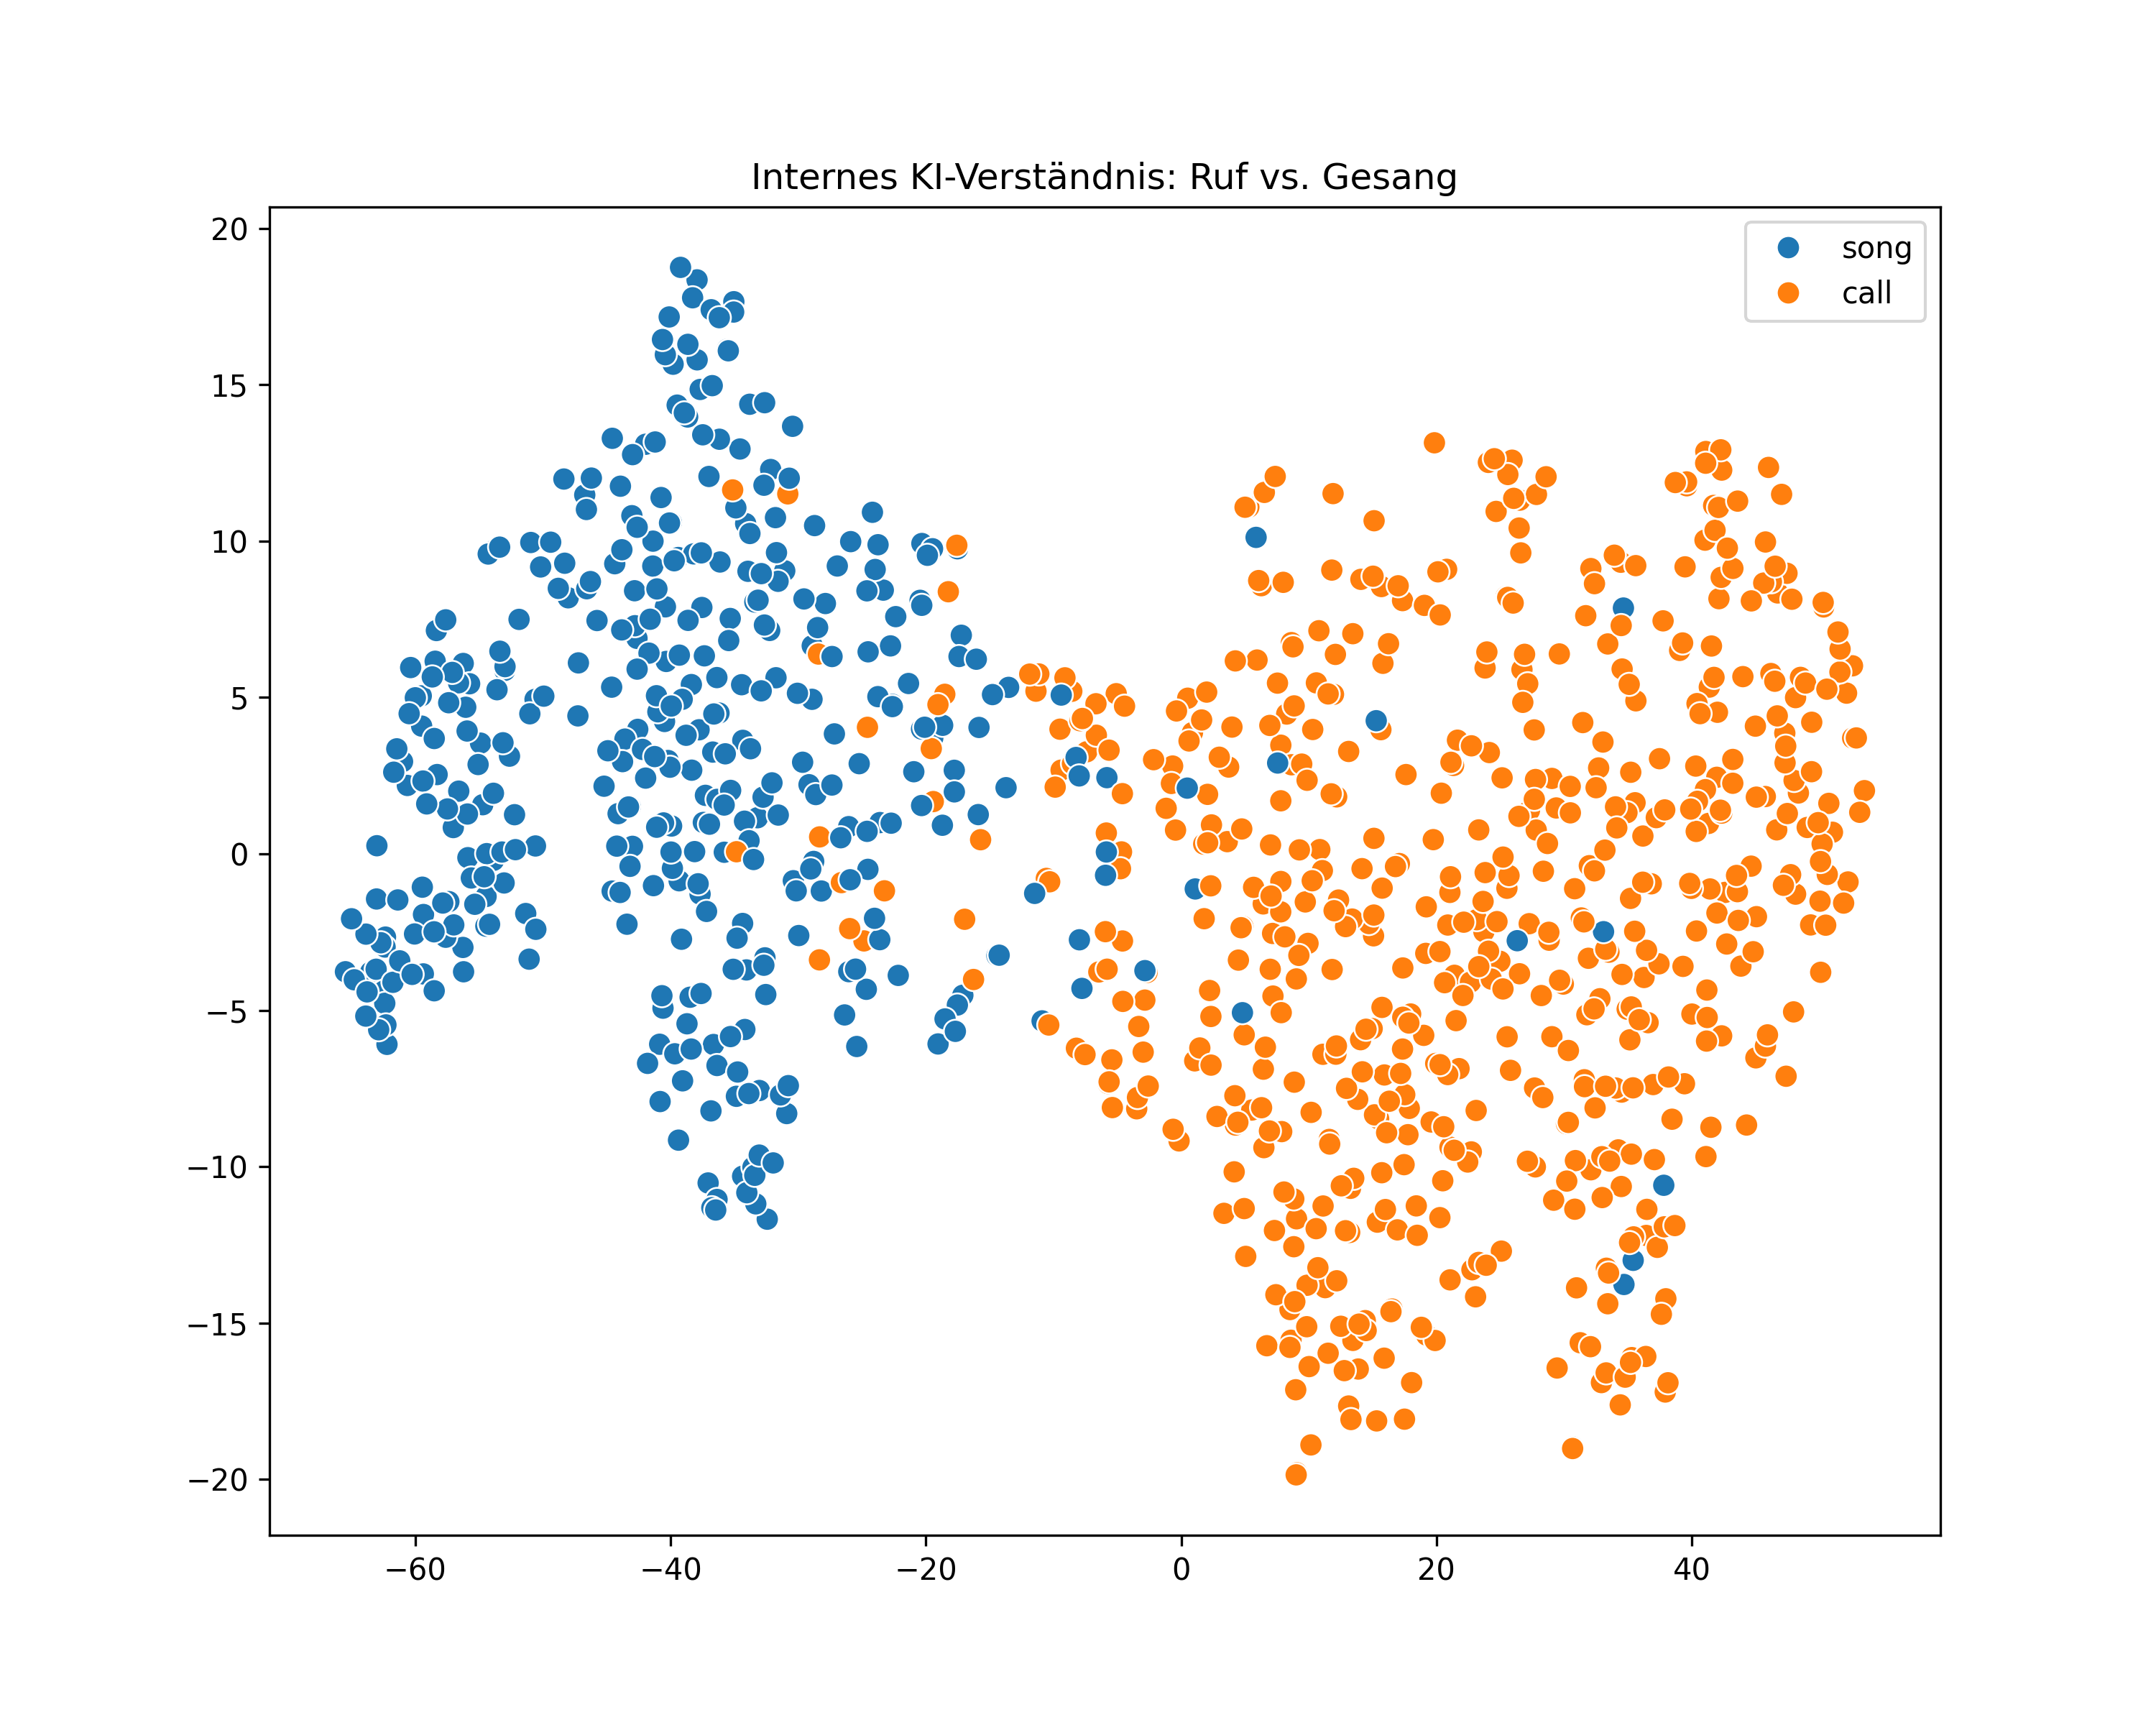
\includegraphics[width=\textwidth]{../visuals/experiments/europe/tsne_song_vs_call.png}
        \caption{t-SNE Visualisierung: Rufe (Call) und Gesänge (Song) bilden separate Cluster.}
    \end{subfigure}
    \hfill
    \begin{subfigure}[b]{0.51\textwidth}
        \centering
        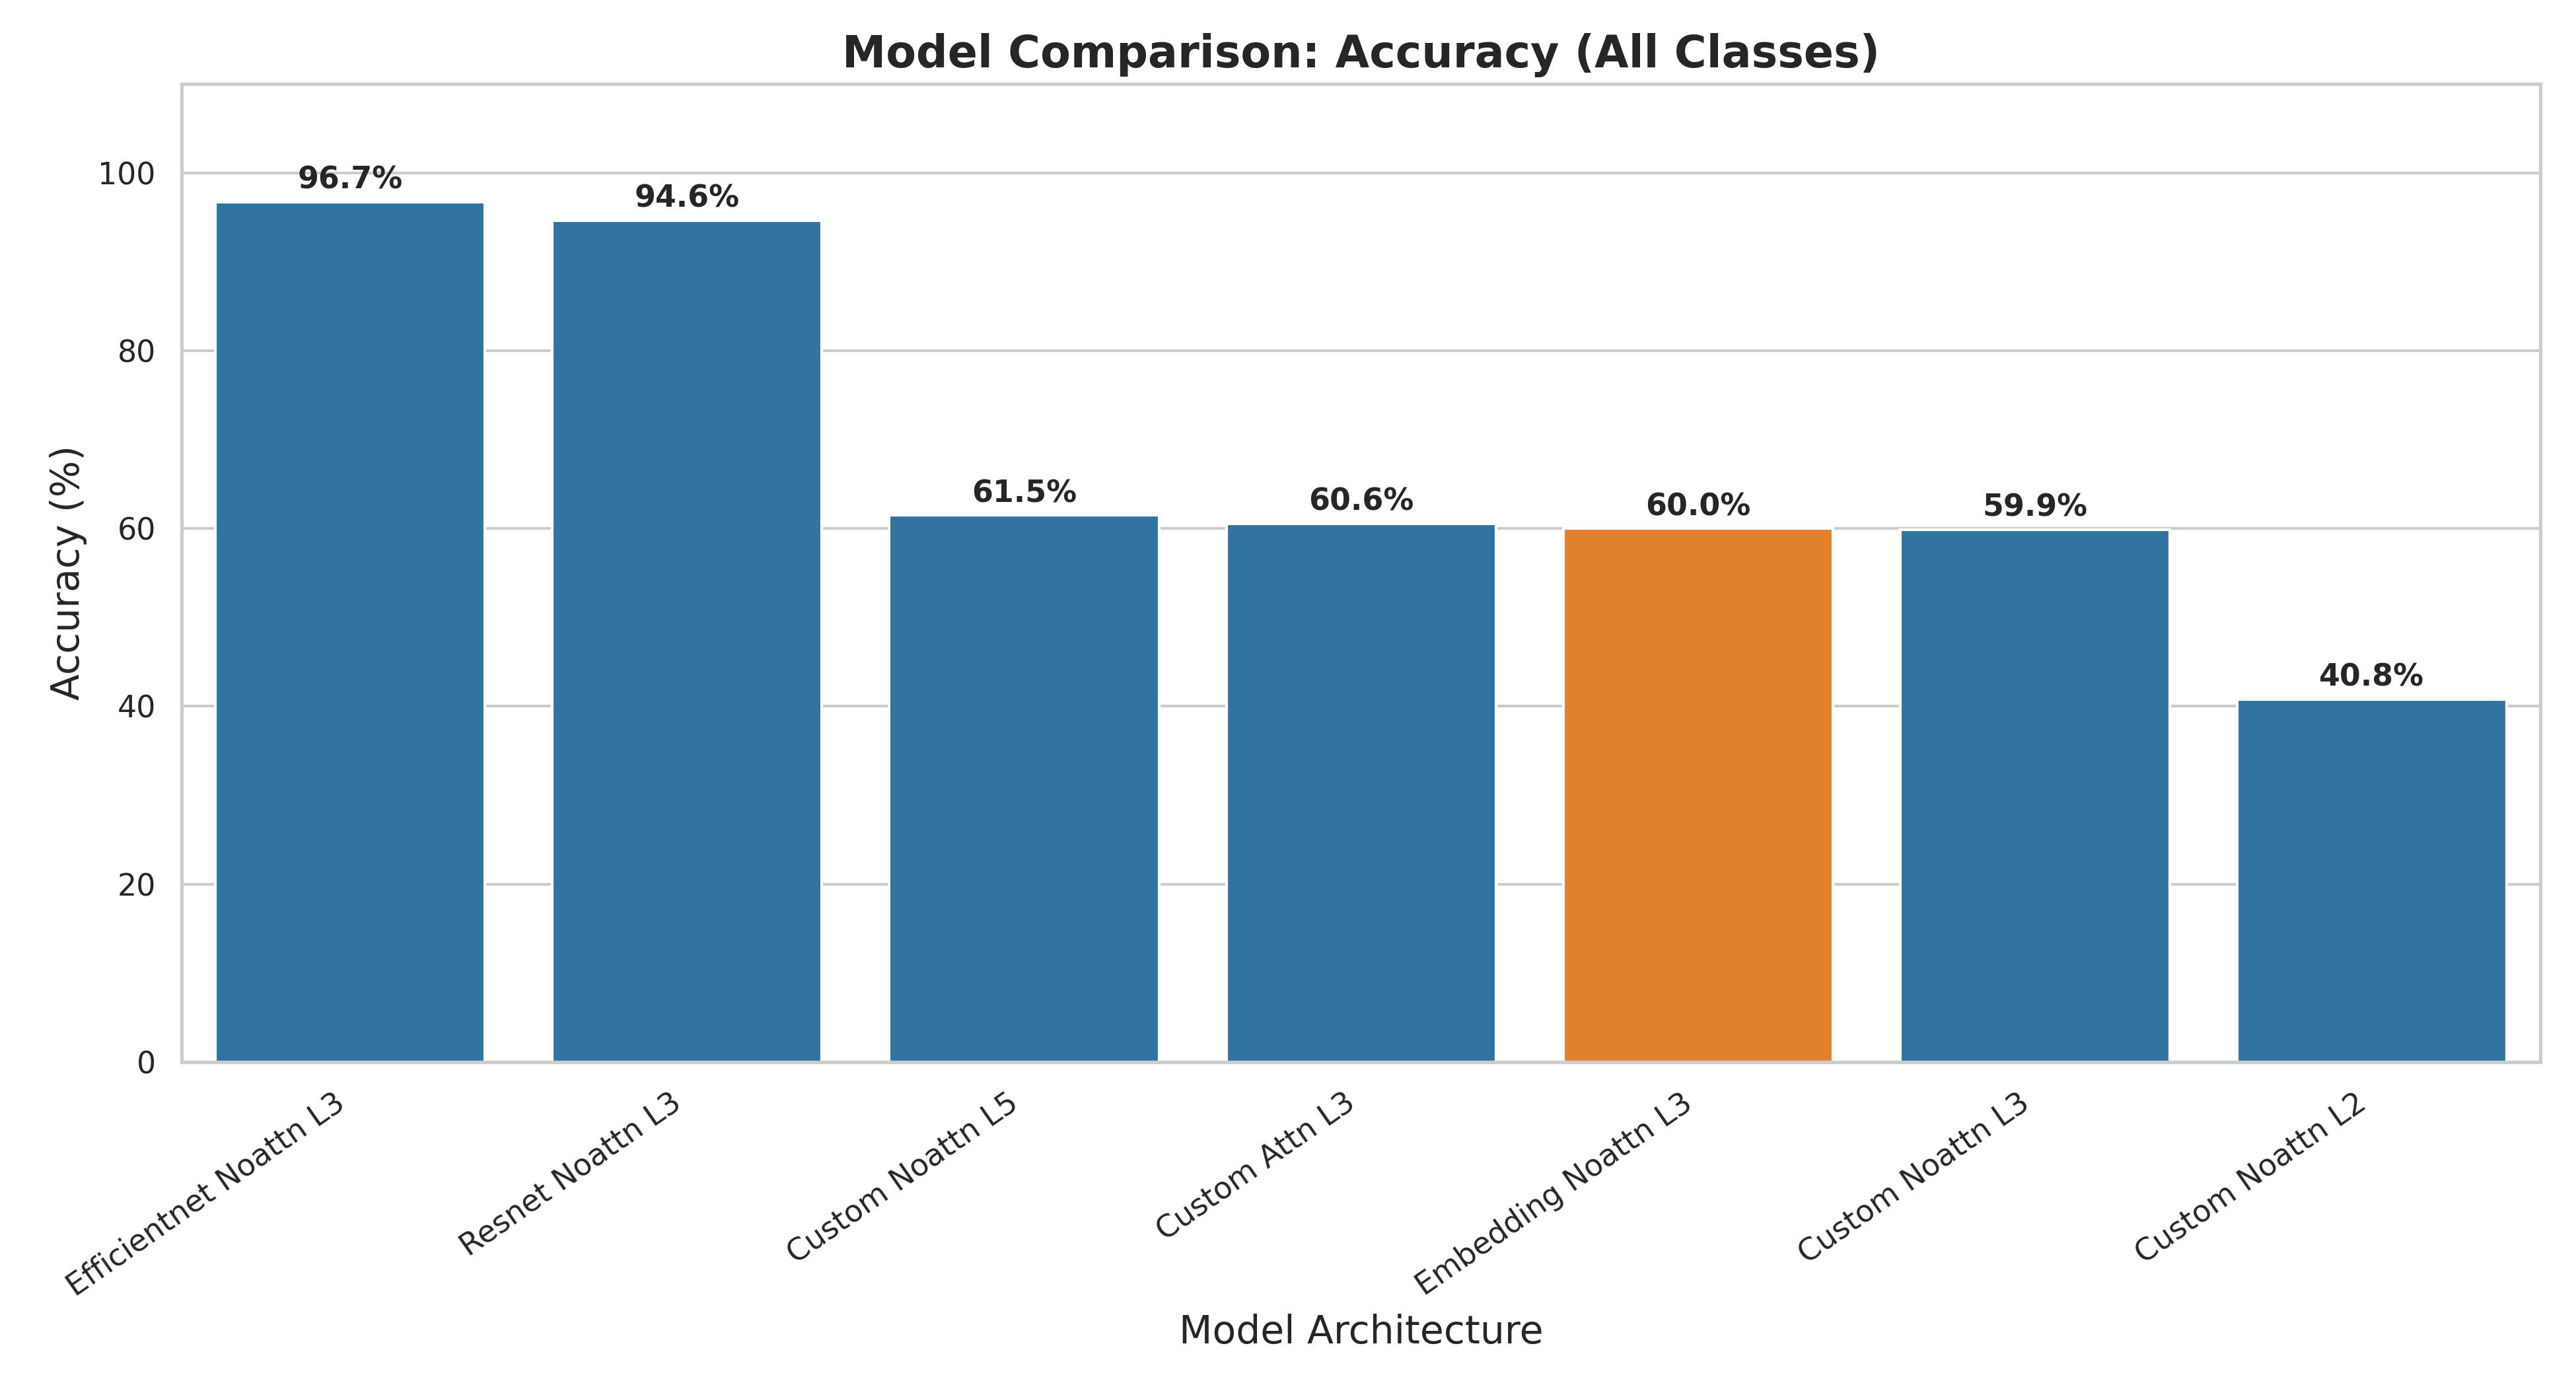
\includegraphics[width=\textwidth]{../visuals/experiments/europe/sliding_window_comparison_updated.png}
        \caption{Vergleich der Accuracy über alle untersuchten KI-Architekturen hinweg.}
    \end{subfigure}
    \caption{Zusatzexperimente: Interne Repräsentation und Modellskalierung.}
    \label{fig:tsne}
\end{figure}

\subsection{Sliding Window Inference \& Grad-CAM}
Im operativen Einsatz analysiert das Modell einen endlosen Audio-Stream durch ein sich verschiebendes \enquote{Sliding Window}. Mittels \textit{Grad-CAM} (Gradient-weighted Class Activation Mapping) konnten wir verifizieren, dass das Modell tatsächlich auf die artspezifischen Frequenzmodulationen im Gesang achtet und Hintergrundrauschen ignoriert (siehe rote/gelbe Bereiche in Abb. \ref{fig:sliding}).

\begin{figure}[H]
    \centering
    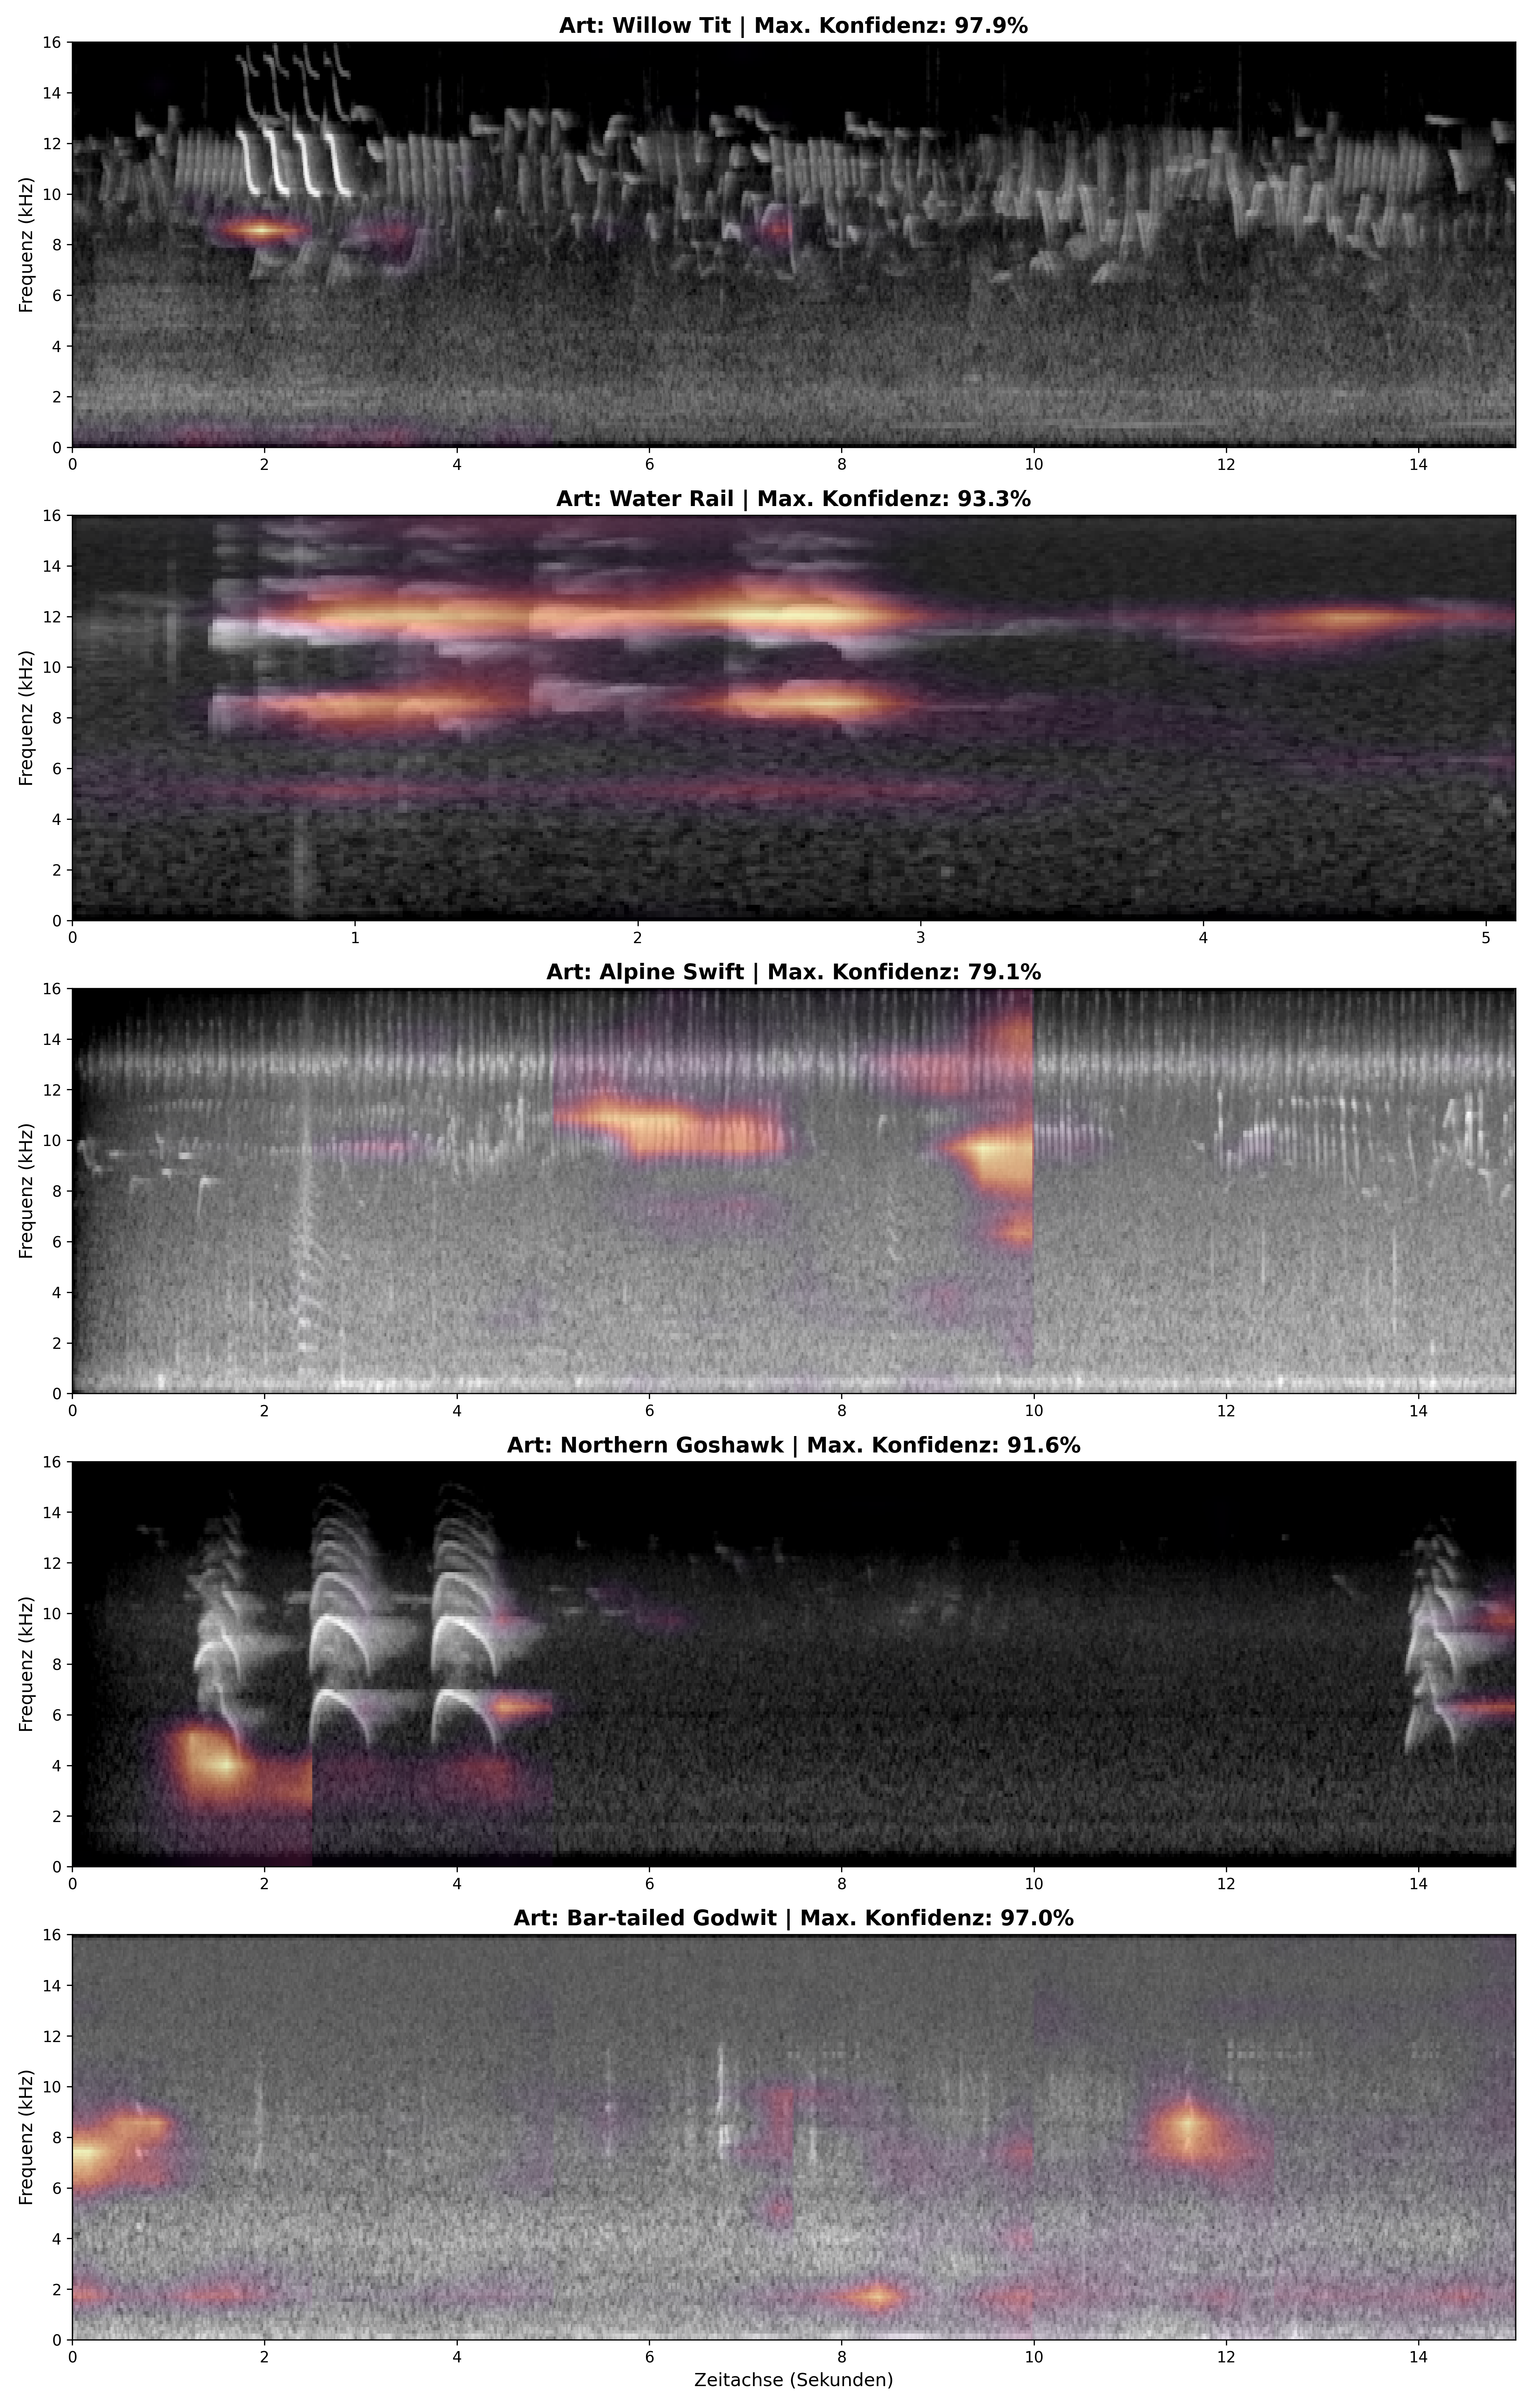
\includegraphics[width=\textwidth, height=0.45\textheight, keepaspectratio]{../visuals/experiments/europe/gradcam_sliding_window.png}
    \caption{Grad-CAM Visualisierung: Die Heatmap markiert hochpräzise die Frequenzmuster, die das neuronale Netz zur Entscheidungsfindung herangezogen hat.}
    \label{fig:sliding}
\end{figure}

\subsection{Algorithmische Signalstabilisierung (Post-Processing)}
Im realen Wald verfälschen Windböen oder knackende Äste kurzzeitig das Mikrofonsignal. Dies führt bei der KI-Auswertung zu Fehlalarmen (False Positives) oder kurzen Erkennungslücken (False Negatives). Wir lösten dieses Problem durch zwei rechenleichte mathematische Post-Processing-Techniken, ohne das Modell neu trainieren zu müssen:

\textbf{1. Temporale Glättung (Test-Time Augmentation):}
Wir legen eine mathematische 1D-Faltung (Kernel: \texttt{[0.1, 0.2, 0.4, 0.2, 0.1]}) über die Zeitachse. Die Vorhersage eines 5-Sekunden-Fensters wird dadurch durch die vorherigen und nachfolgenden Fenster gestützt. Kurze Konfidenzeinbrüche werden so effektiv geglättet (Abb. \ref{fig:smoothing}).

\begin{figure}[H]
    \centering
    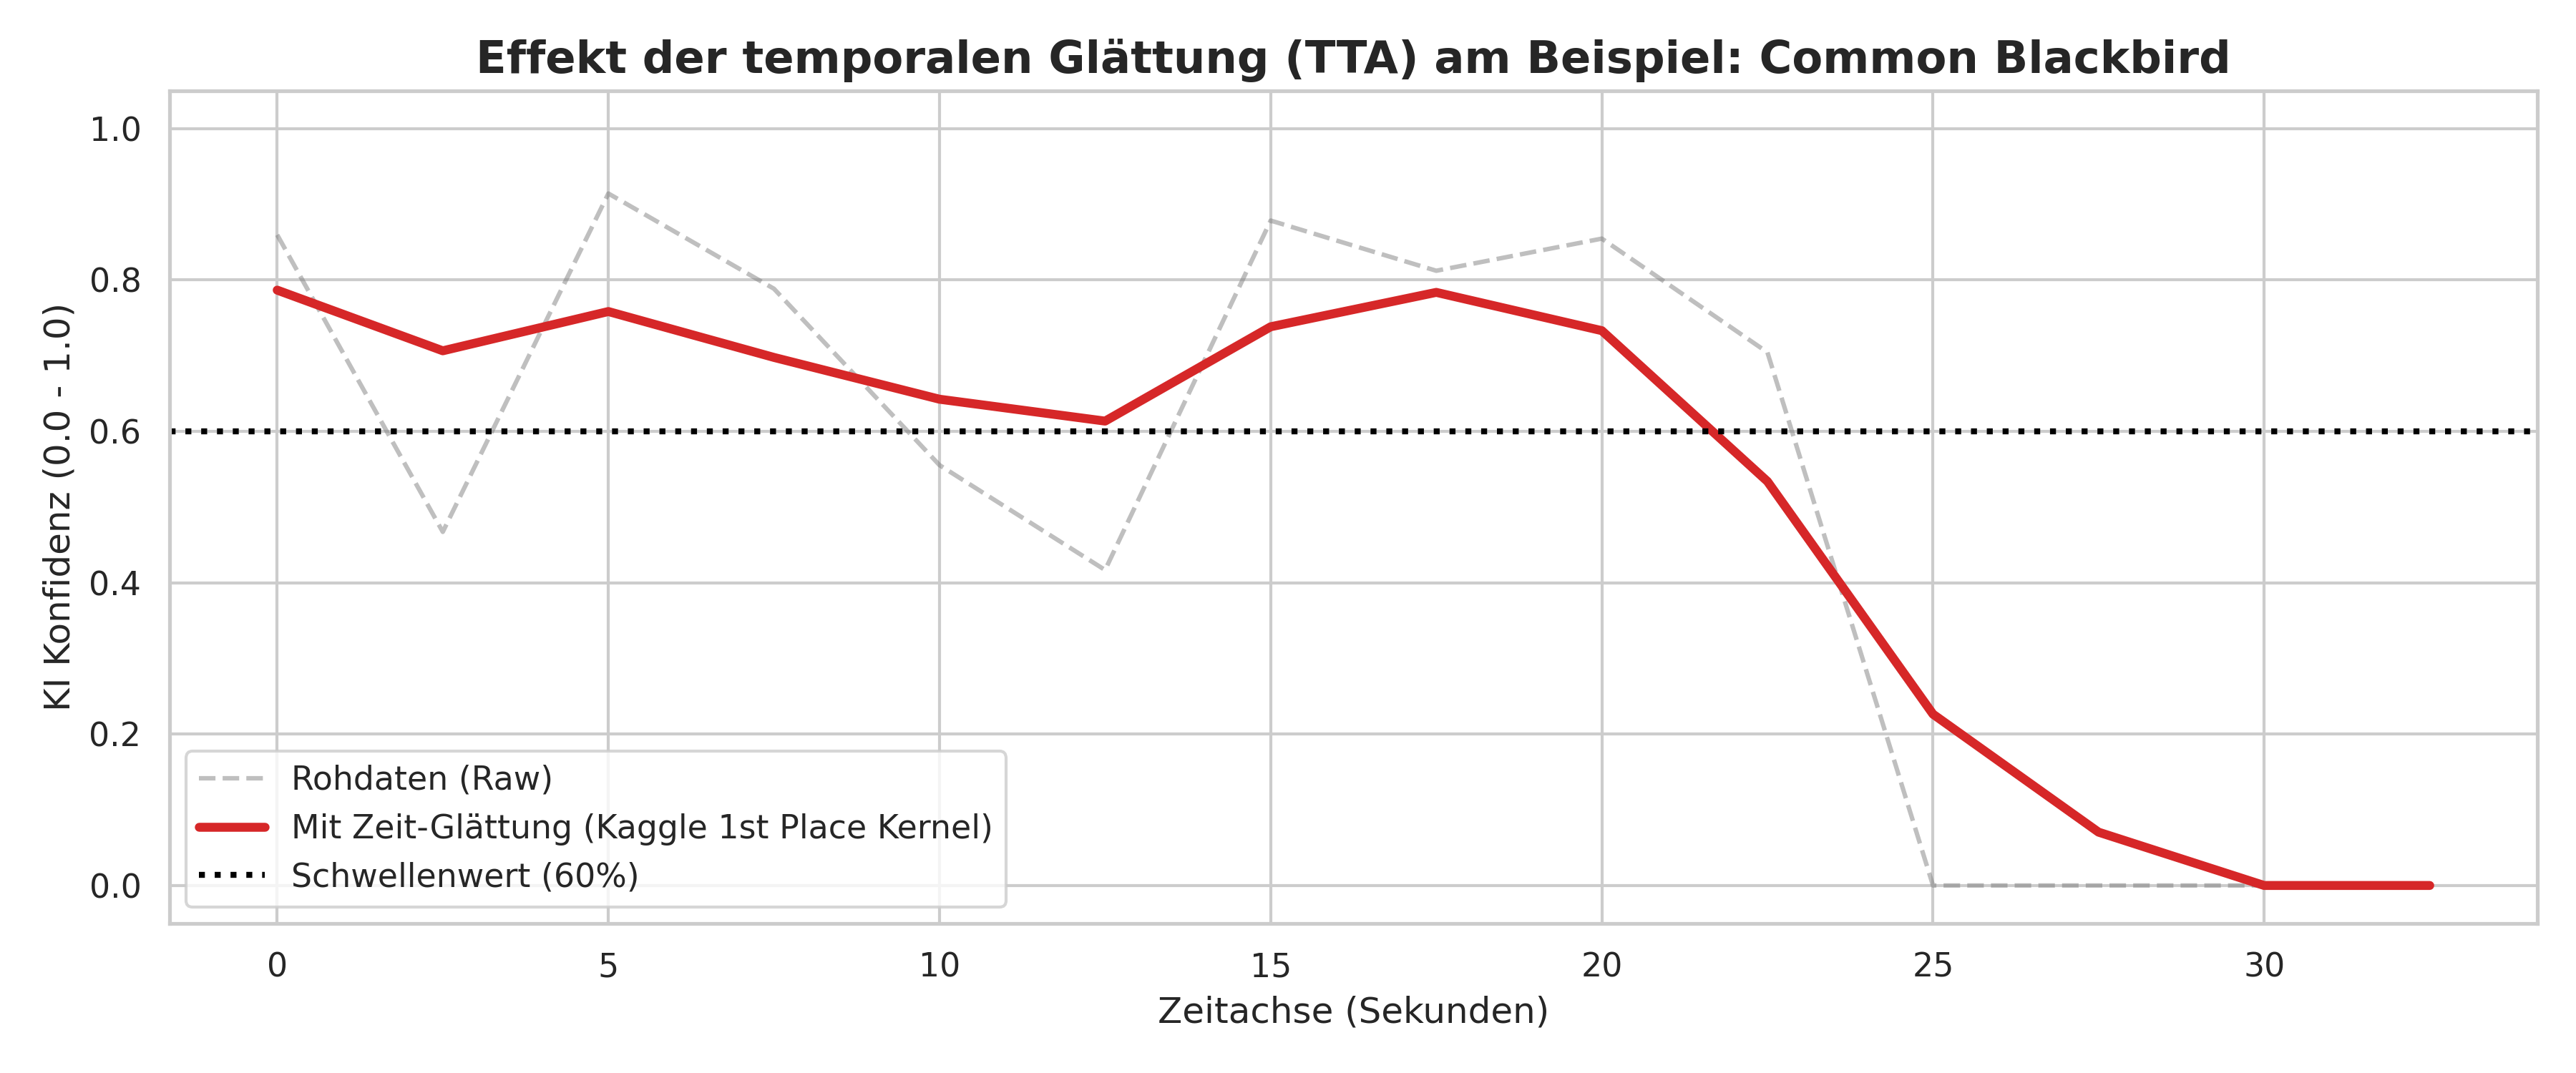
\includegraphics[width=0.9\textwidth]{../visuals/experiments/smoothing_comparison.png}
    \caption{Temporale Glättung: Durch den Einbezug benachbarter Zeitfenster wird das stark schwankende Rohsignal stabilisiert. Lücken in der Erkennung werden verhindert.}
    \label{fig:smoothing}
\end{figure}

\textbf{2. Root-Scaled Context Suppression:}
Um isolierte Fehlalarme zu filtern, nutzen wir die Annahme, dass ein echter Vogel innerhalb einer Aufnahme mindestens einmal einen sehr deutlichen \enquote{Anker-Ruf} abgibt. Fehlt dieser globale Maximalwert in der Datei, handelt es sich meist um Rauschen. Statt die Vorhersagen linear mit dem globalen Maximalwert zu multiplizieren, haben wir eine verbesserte Formel entwickelt. Wir multiplizieren die Wahrscheinlichkeit $P(t, c)$ jedes Fensters mit der Wurzel des klassenspezifischen Maximalwerts ($\sqrt{P_{max}}$). Dies dämpft isolierte Fehlalarme extrem zuverlässig unter die Erkennungsschwelle, erhält aber leisere, echte Rufe von weiter entfernten Vögeln (Abb. \ref{fig:fpsuppression}).

\begin{figure}[H]
    \centering
    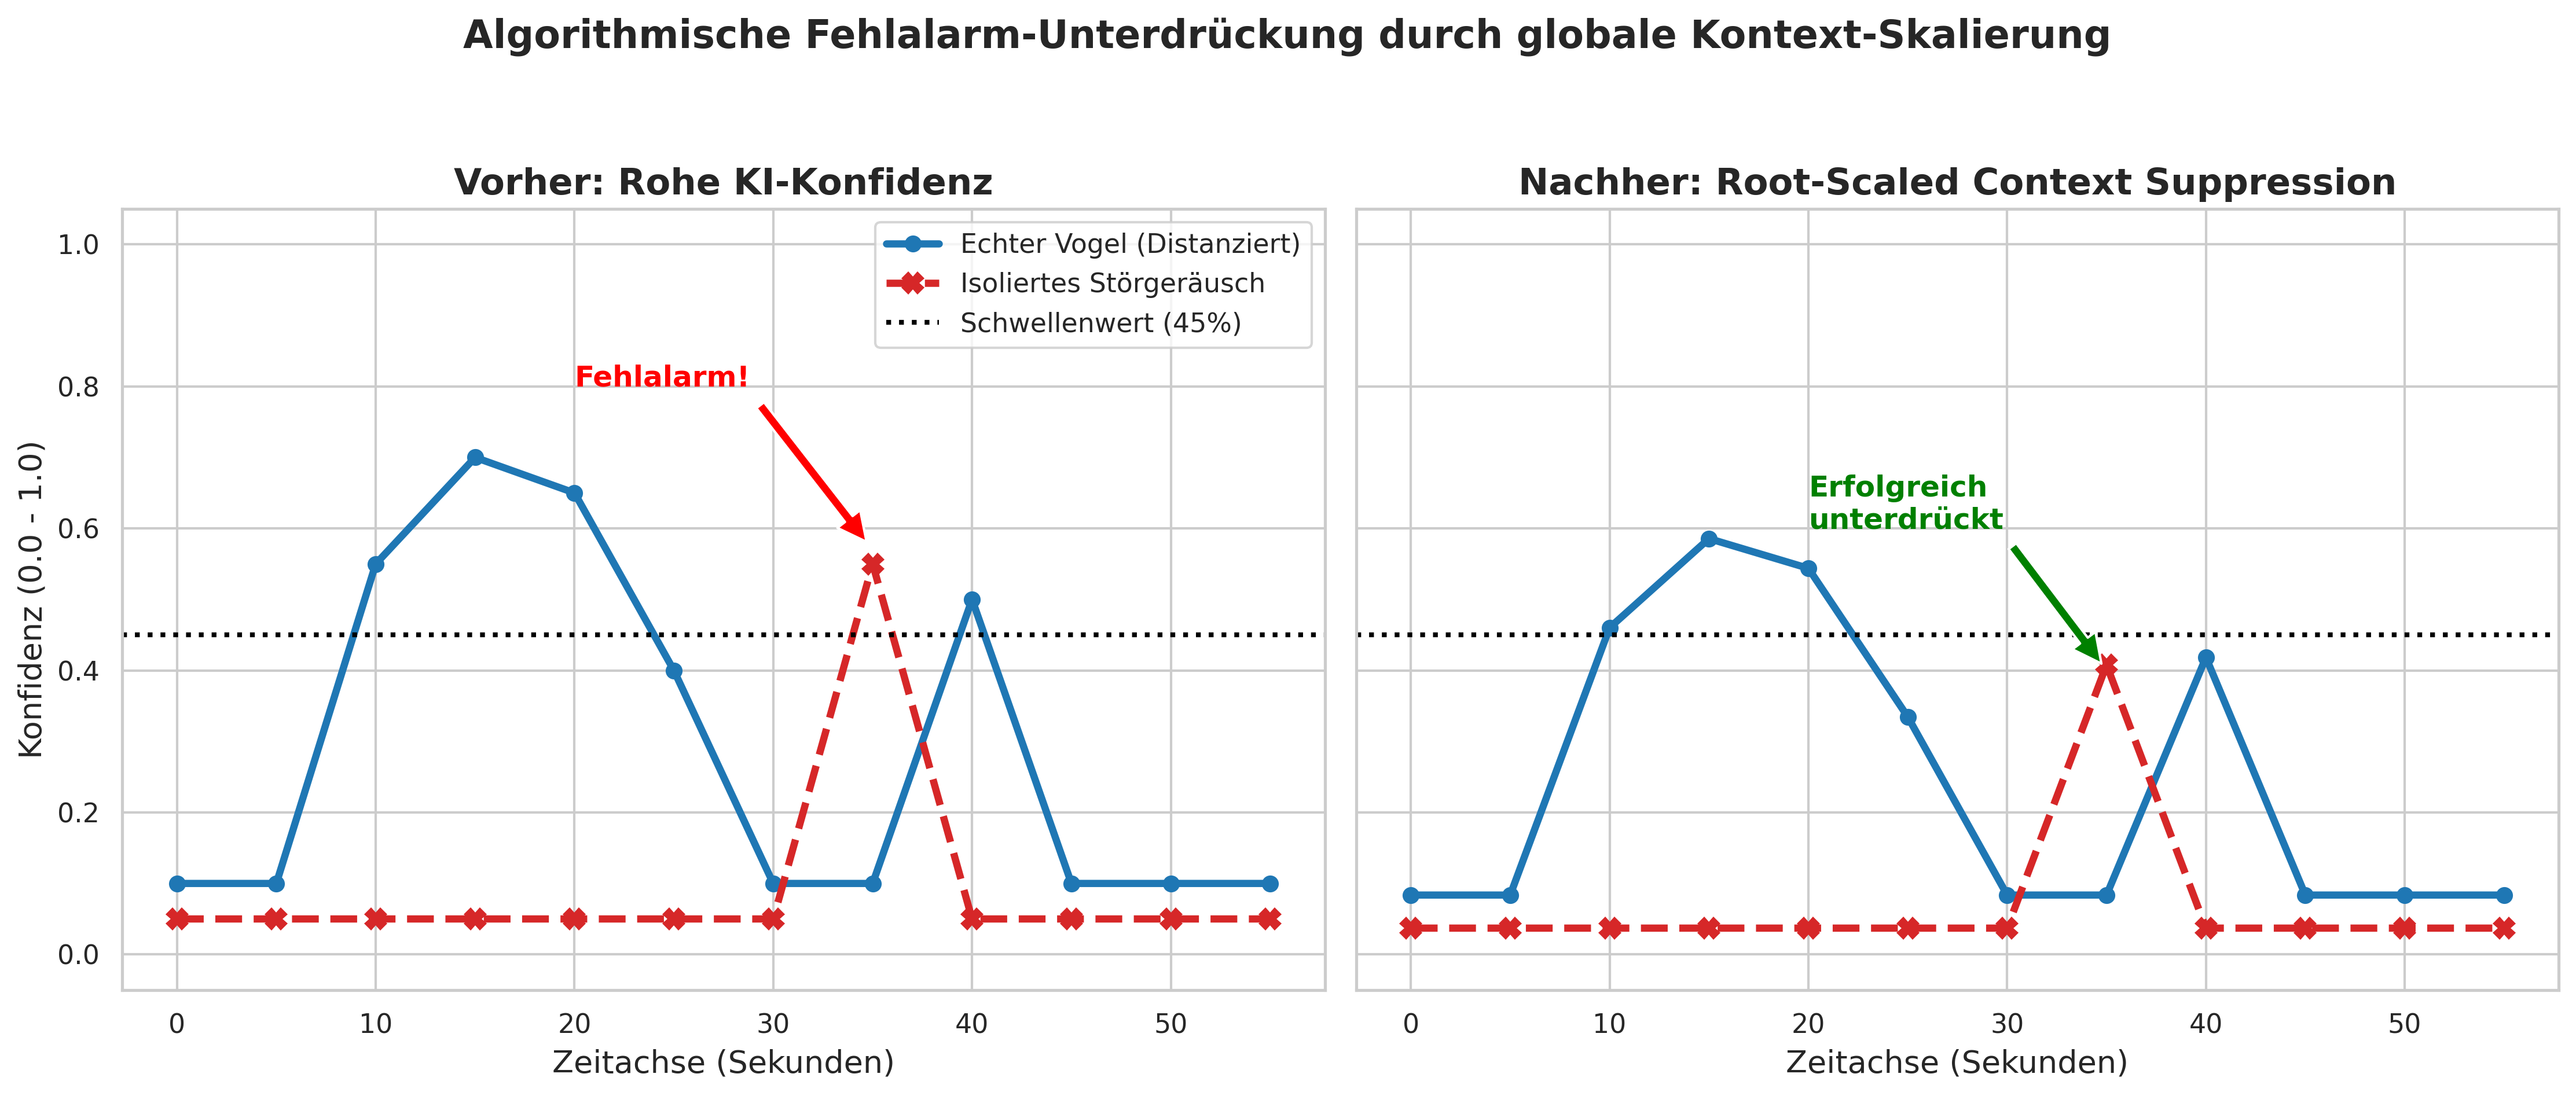
\includegraphics[width=0.9\textwidth]{../visuals/experiments/false_positive_suppression.png}
    \caption{Root-Scaled Suppression: Der isolierte Fehlalarm (rot) ohne starken globalen Anker stürzt unter den Schwellenwert ab, während der echte Ruf (blau) intakt bleibt.}
    \label{fig:fpsuppression}
\end{figure}

\section{Hardware-Design und Edge-Deployment}
Die KI-Software läuft auf einem \textit{Raspberry Pi Zero 2 W}, eingefasst in ein modulares, am CAD entworfenes Gehäuse mit integriertem Solarpanel und akustischem Mikrofon-Trichter (Abb. \ref{fig:hardware}). Da die Hardware stark ressourcenbeschränkt ist (512\,MB RAM, schwache CPU), führten wir zwei wesentliche Software-Hardware-Optimierungen durch.

\begin{figure}[H]
    \centering
    \begin{subfigure}[b]{0.32\textwidth}
        \centering
        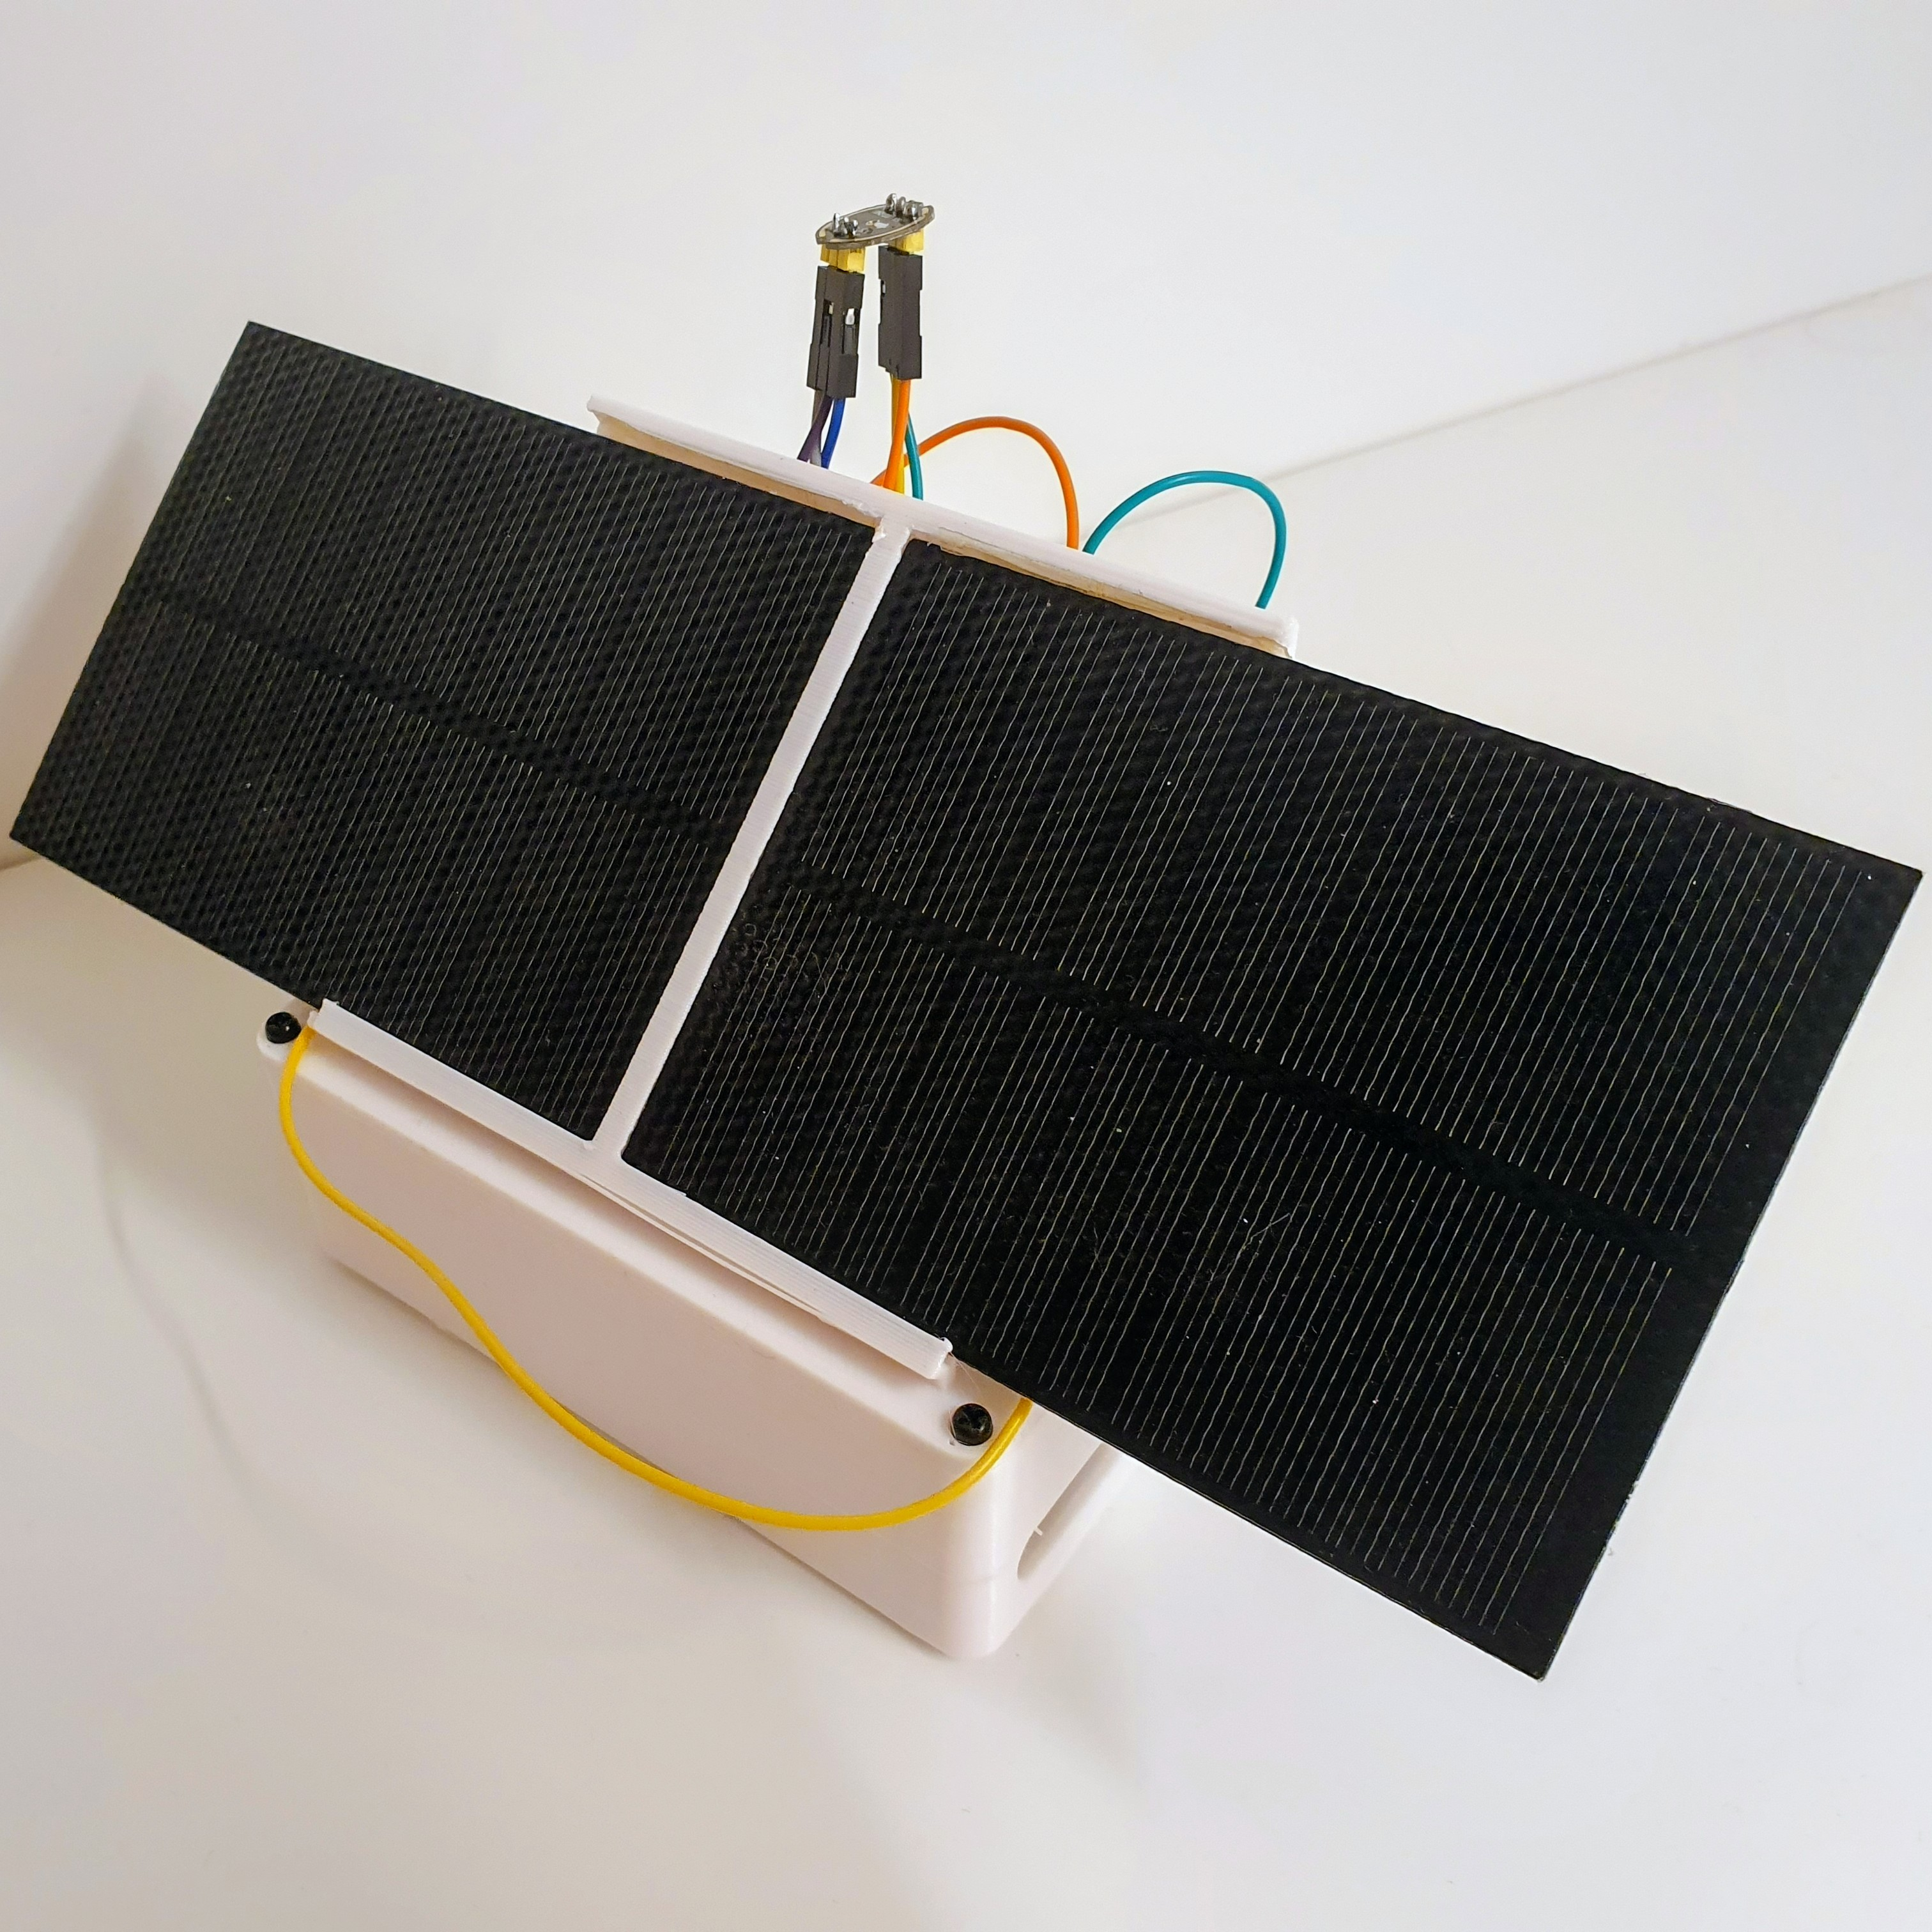
\includegraphics[width=\textwidth]{../visuals/cad/RealView.jpg}
        \caption{Zusammengebaut}
    \end{subfigure}
    \hfill
    \begin{subfigure}[b]{0.32\textwidth}
        \centering
        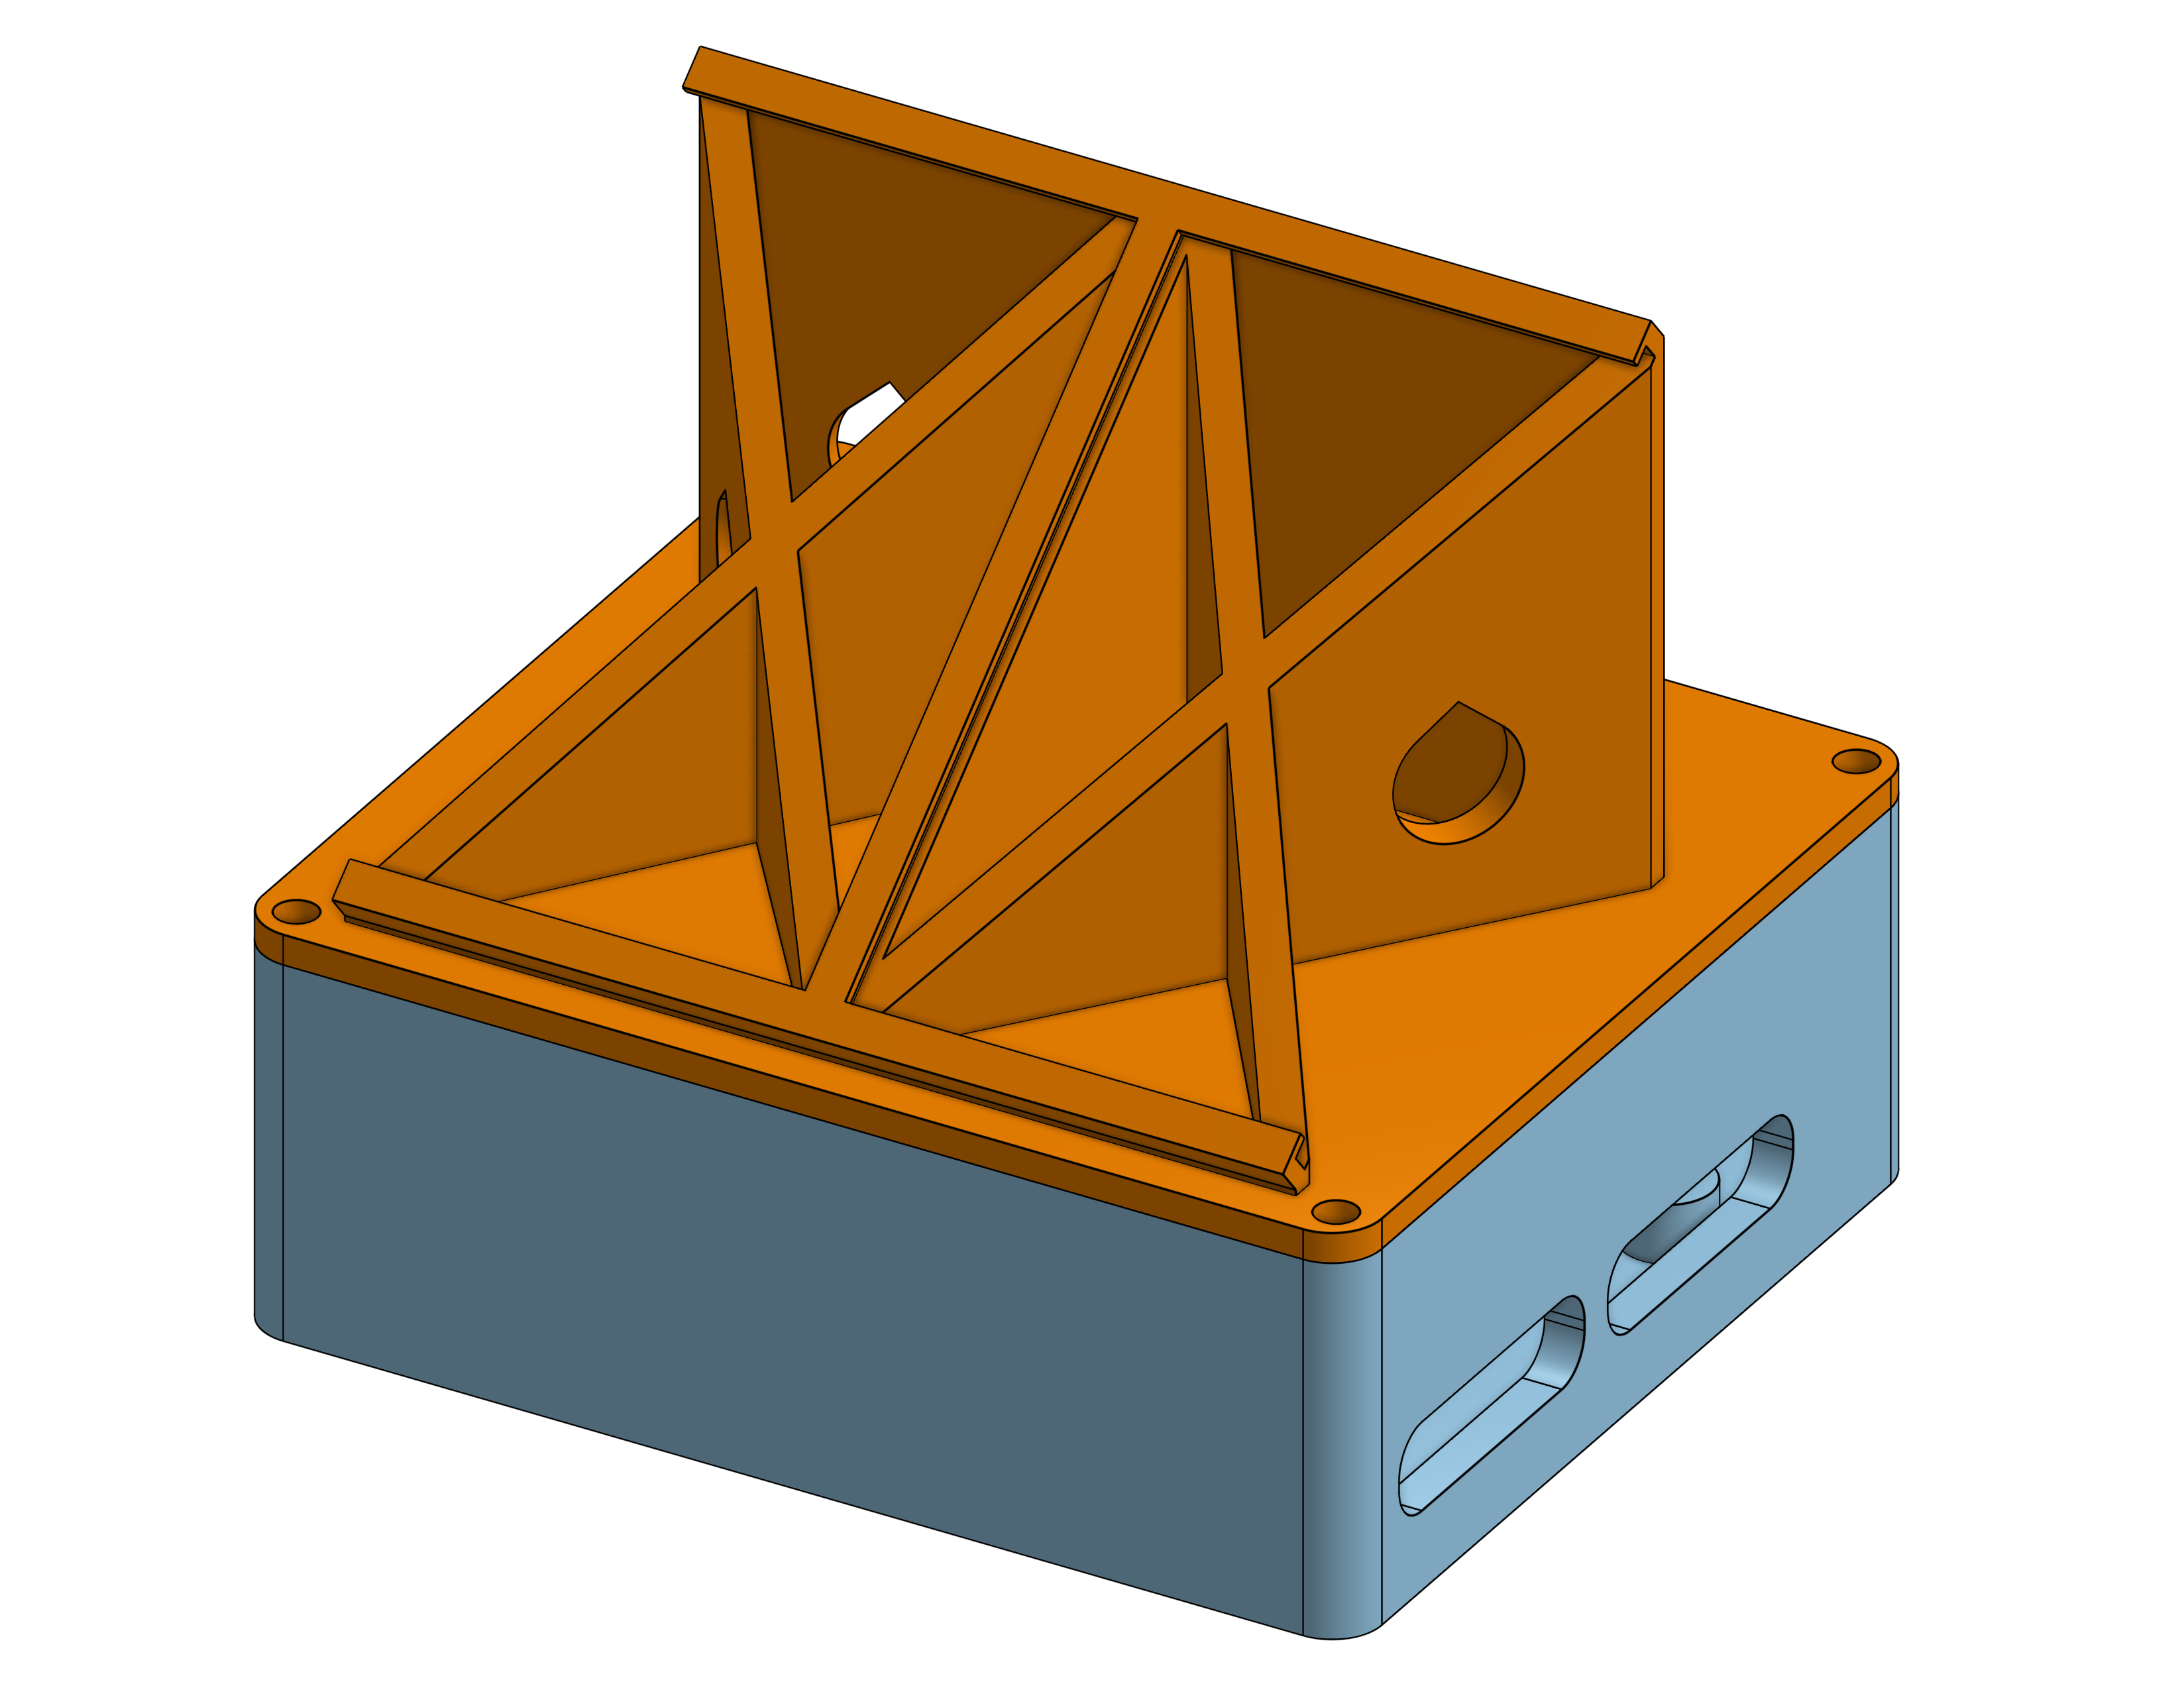
\includegraphics[width=\textwidth]{../visuals/cad/OnshapeModelView_OnlyCasing.png}
        \caption{Gehäuse-Struktur}
    \end{subfigure}
    \hfill
    \begin{subfigure}[b]{0.32\textwidth}
        \centering
        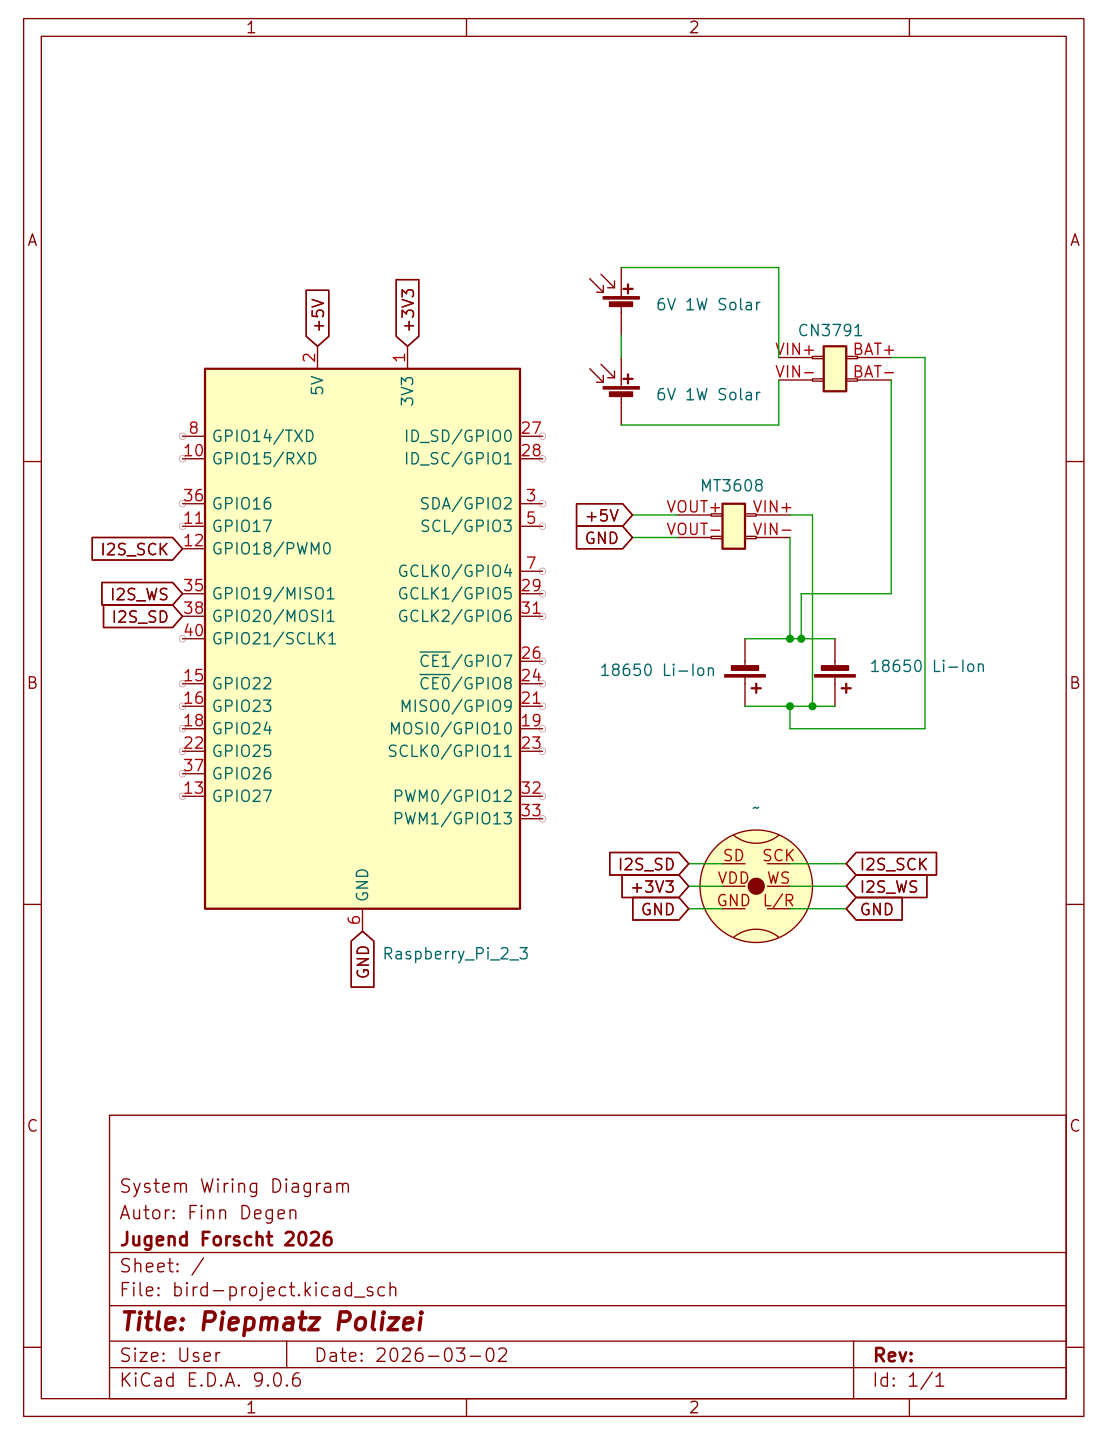
\includegraphics[width=\textwidth]{../visuals/electronics/schematic.png}
        \caption{Elektronik-Schaltplan}
    \end{subfigure}
    \caption{Unsere CAD-Konstruktion und das Schaltungsdesign für den autonomen Feldeinsatz.}
    \label{fig:hardware}
\end{figure}

\subsection{Architektur-Evaluation: MobileNetV3 vs. EfficientNet}

Audio-Spektrogramme liegen als Graustufenbilder vor, während vortrainierte CNNs typischerweise 3-Kanal-Eingaben erwarten. Wir testeten daher eine 1-Kanal-Anpassung durch Kompression der Eingabe und Aggregation der Pre-Training-Gewichte, um Speicherbandbreite zu sparen.

Zwar verbesserte diese Variante bei EfficientNet die CPU-Latenz deutlich – unter anderem durch bessere Cache-Nutzung –, jedoch ging dies mit einem spürbaren Genauigkeitsverlust einher.

Als bessere Lösung erwies sich der Wechsel der Architektur: \textbf{MobileNetV3-Small}, speziell für schwache Hardware optimiert, erreichte im unveränderten 3-Kanal-Modus eine deutlich schnellere Inferenz bei gleichzeitig hoher Accuracy. Damit wurde MobileNetV3 zur bevorzugten Architektur für das Edge-Deployment.

\begin{figure}[h]
    \centering
    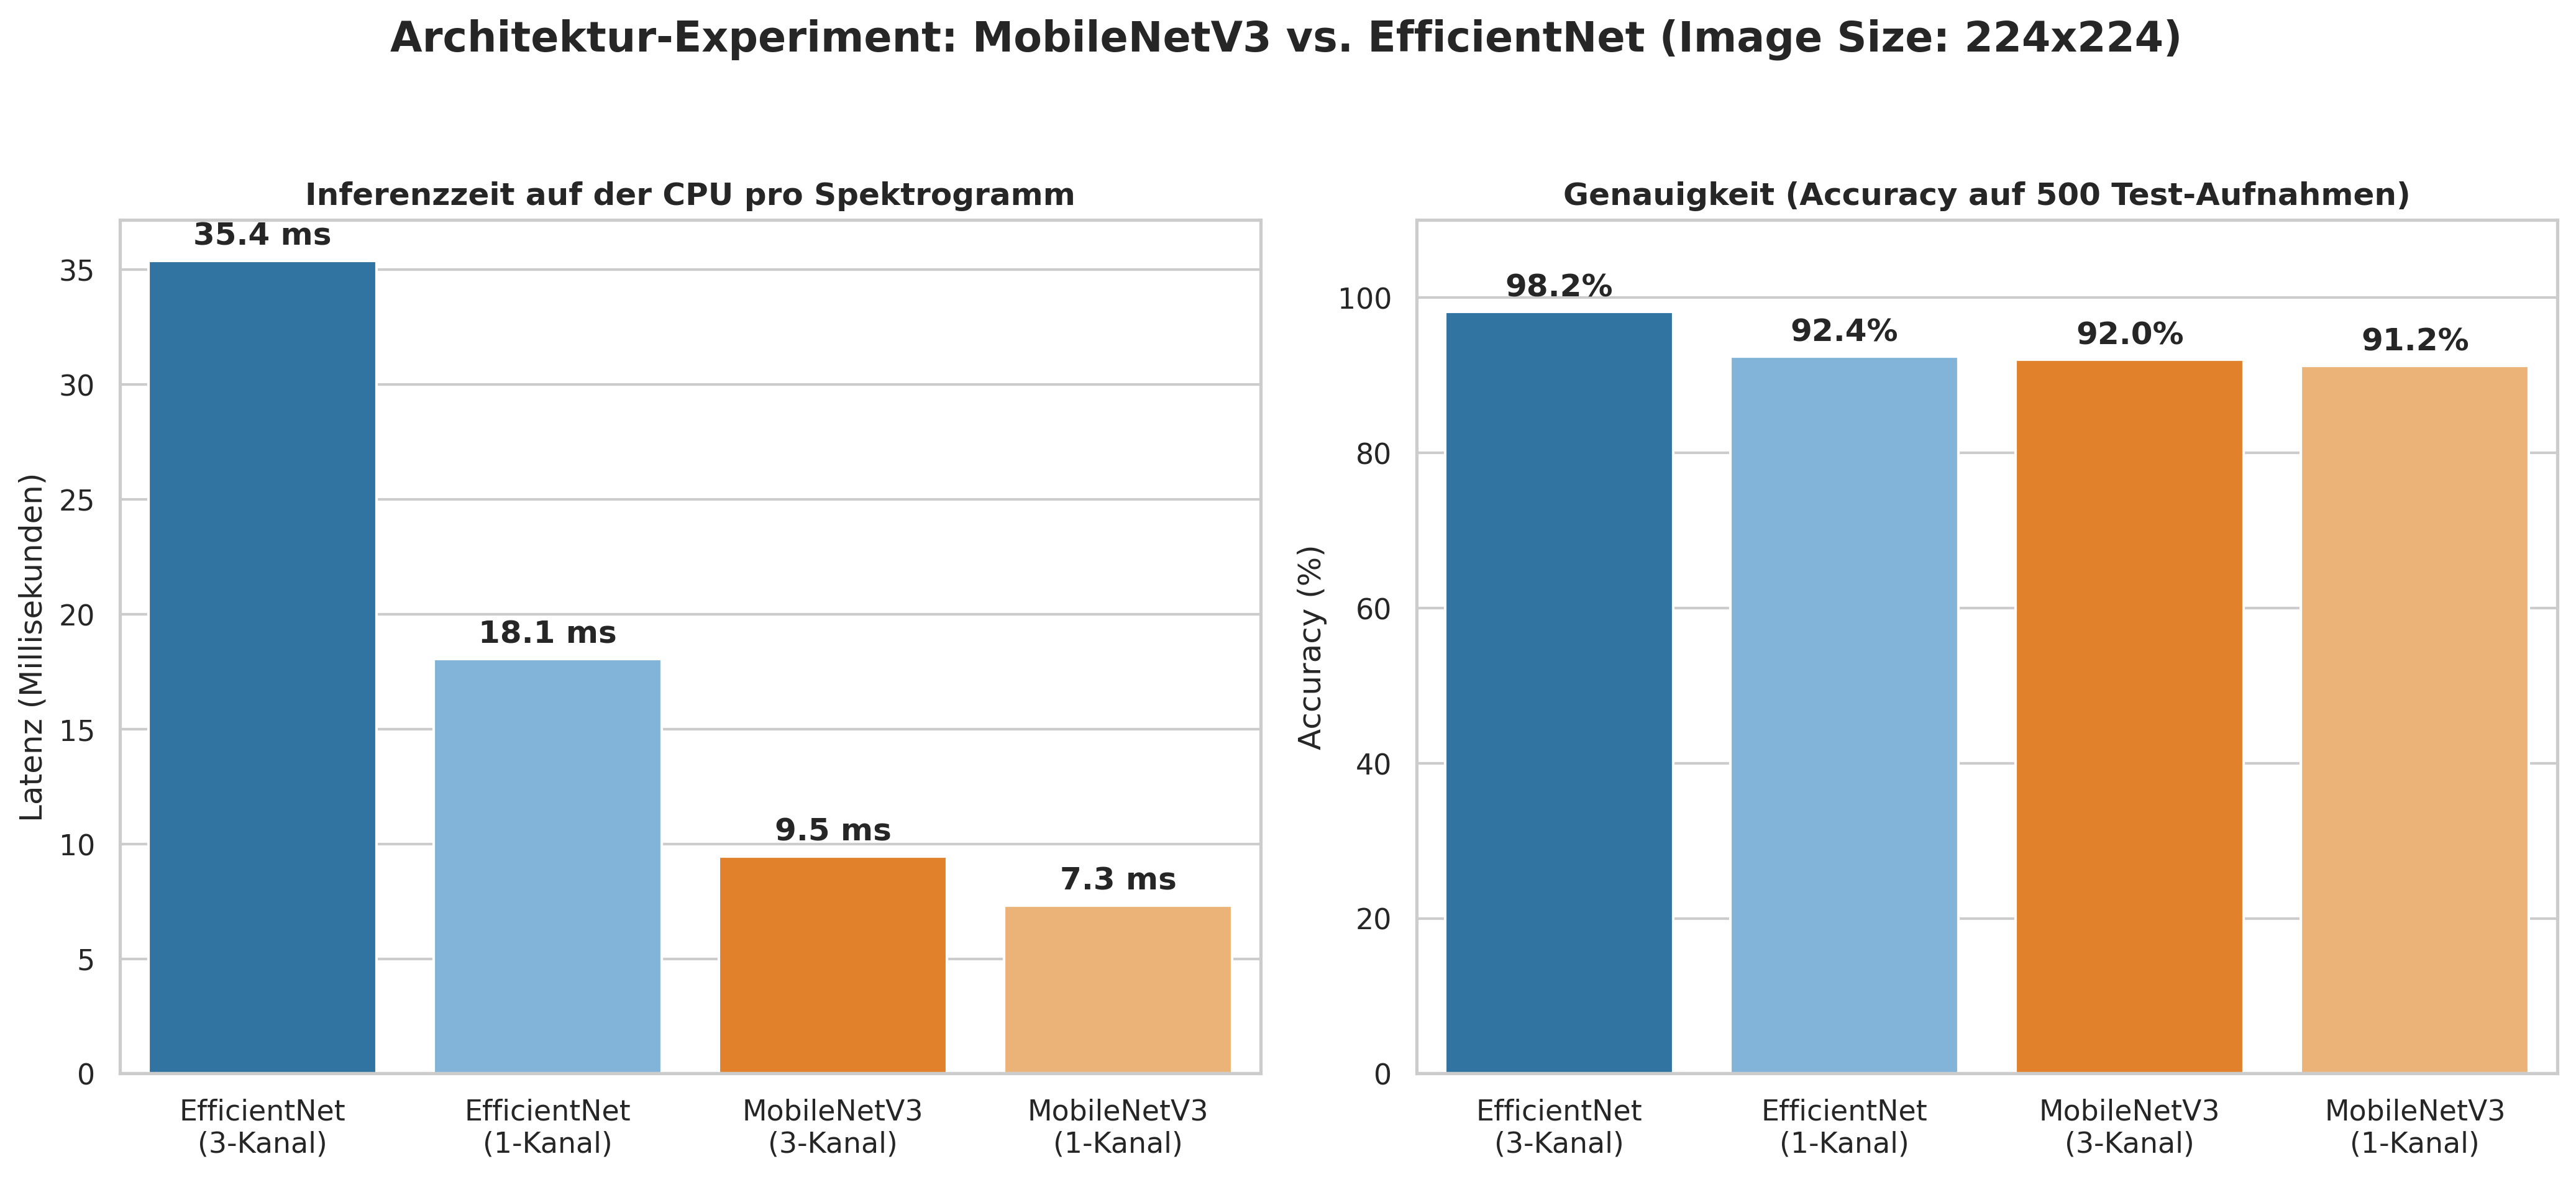
\includegraphics[width=0.8\linewidth]{../visuals/experiments/architecture_speed_comparison.png}
    \caption{Vergleich der Inferenzgeschwindigkeit und Genauigkeit verschiedener Architekturen}
\end{figure}

\subsection{Quantisierungs-Experimente (ONNX)}
Wir wandelten das PyTorch-Modell in das optimierte ONNX-Format \cite{onnx} um und testeten eine 8-Bit Post-Training-Quantisierung. Obwohl die Modellgröße von 19,1\,MB auf kompakte 5,2\,MB sank, kollabierte die Genauigkeit bei der INT8-Rundung auf 25\% (Abb. \ref{fig:quantization}). Die Ursache liegt in der Architektur des EfficientNets: Es nutzt \textit{Squeeze-and-Excitation}-Blöcke, die mit extrem feinen Fließkommaskalierungen arbeiten. Da das FP32-Modell problemlos in den Arbeitsspeicher des Pi passt, verzichten wir zugunsten der Genauigkeit auf die Quantisierung, gewannen jedoch wertvolle hardwarenahe Erkenntnisse über architektonische Limits.

\begin{figure}[H]
    \centering
    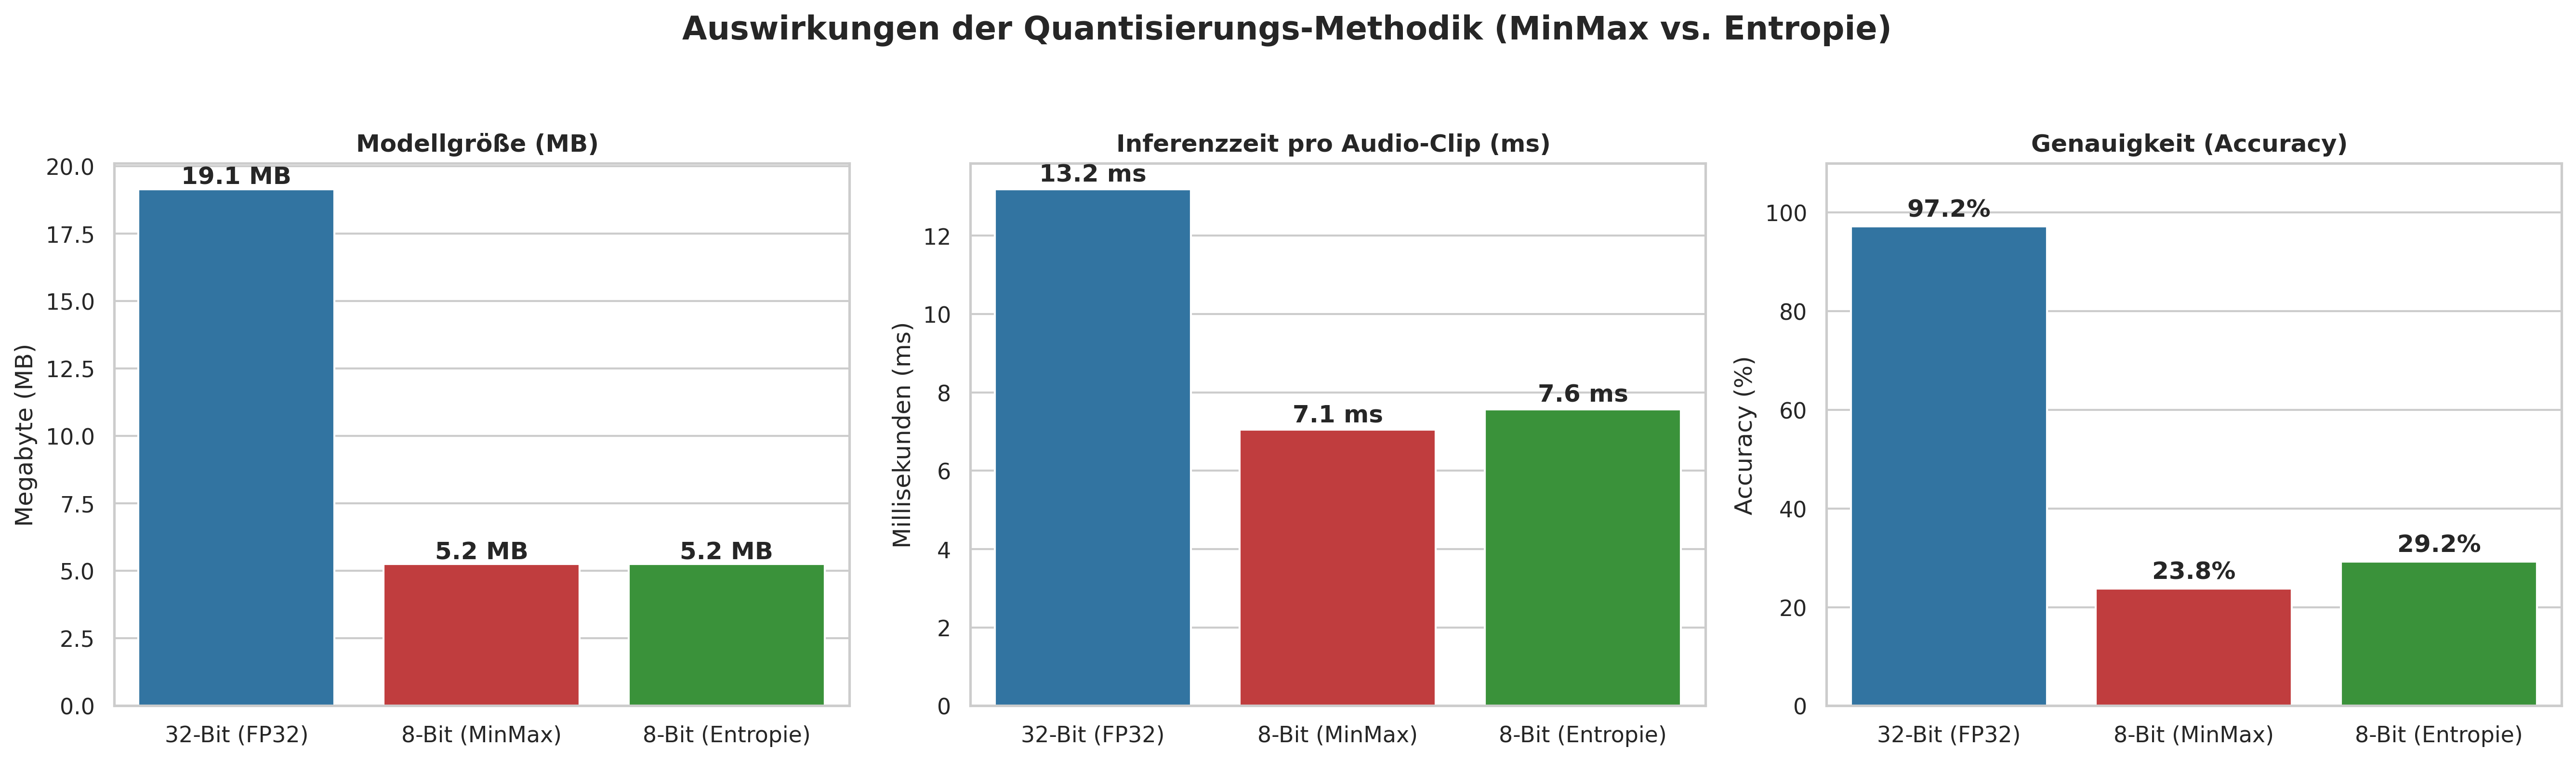
\includegraphics[width=\textwidth]{../visuals/experiments/comparison_quantization.png}
    \caption{Auswertung des Quantisierungs-Experiments: Während die Dateigröße stark schrumpft, führt die komplexe Architektur des EfficientNets bei einer nachträglichen INT8-Konvertierung zu einem massiven und unerwarteten Genauigkeitsverlust.}
    \label{fig:quantization}
\end{figure}

\subsection{Energieeffizienz: Wake-on-Sound Architektur}
Die kontinuierliche Berechnung eines neuronalen Netzes verbraucht massiv Strom. Um die Akkulaufzeit bei schlechtem Wetter zu garantieren, implementierten wir eine heuristische Wake-on-Sound-Vorfilterung ähnlich wie z.B. Sprachassistent Alexa. Der Prozessor berechnet zunächst nur die sehr sparsame RMS-Energie des Mikrofons. Erst wenn ein Schwellenwert überschritten wird (Lärm/Gesang), erwacht das neuronale Netz aus dem Deep-Sleep und berechnet die Inferenz (Abb. \ref{fig:wakeonsound}). Da der Wald nachts und zur Mittagshitze sehr leise ist, sparen wir so bis zu $65\%$ der täglichen Rechenlast.

\begin{figure}[H]
    \centering
    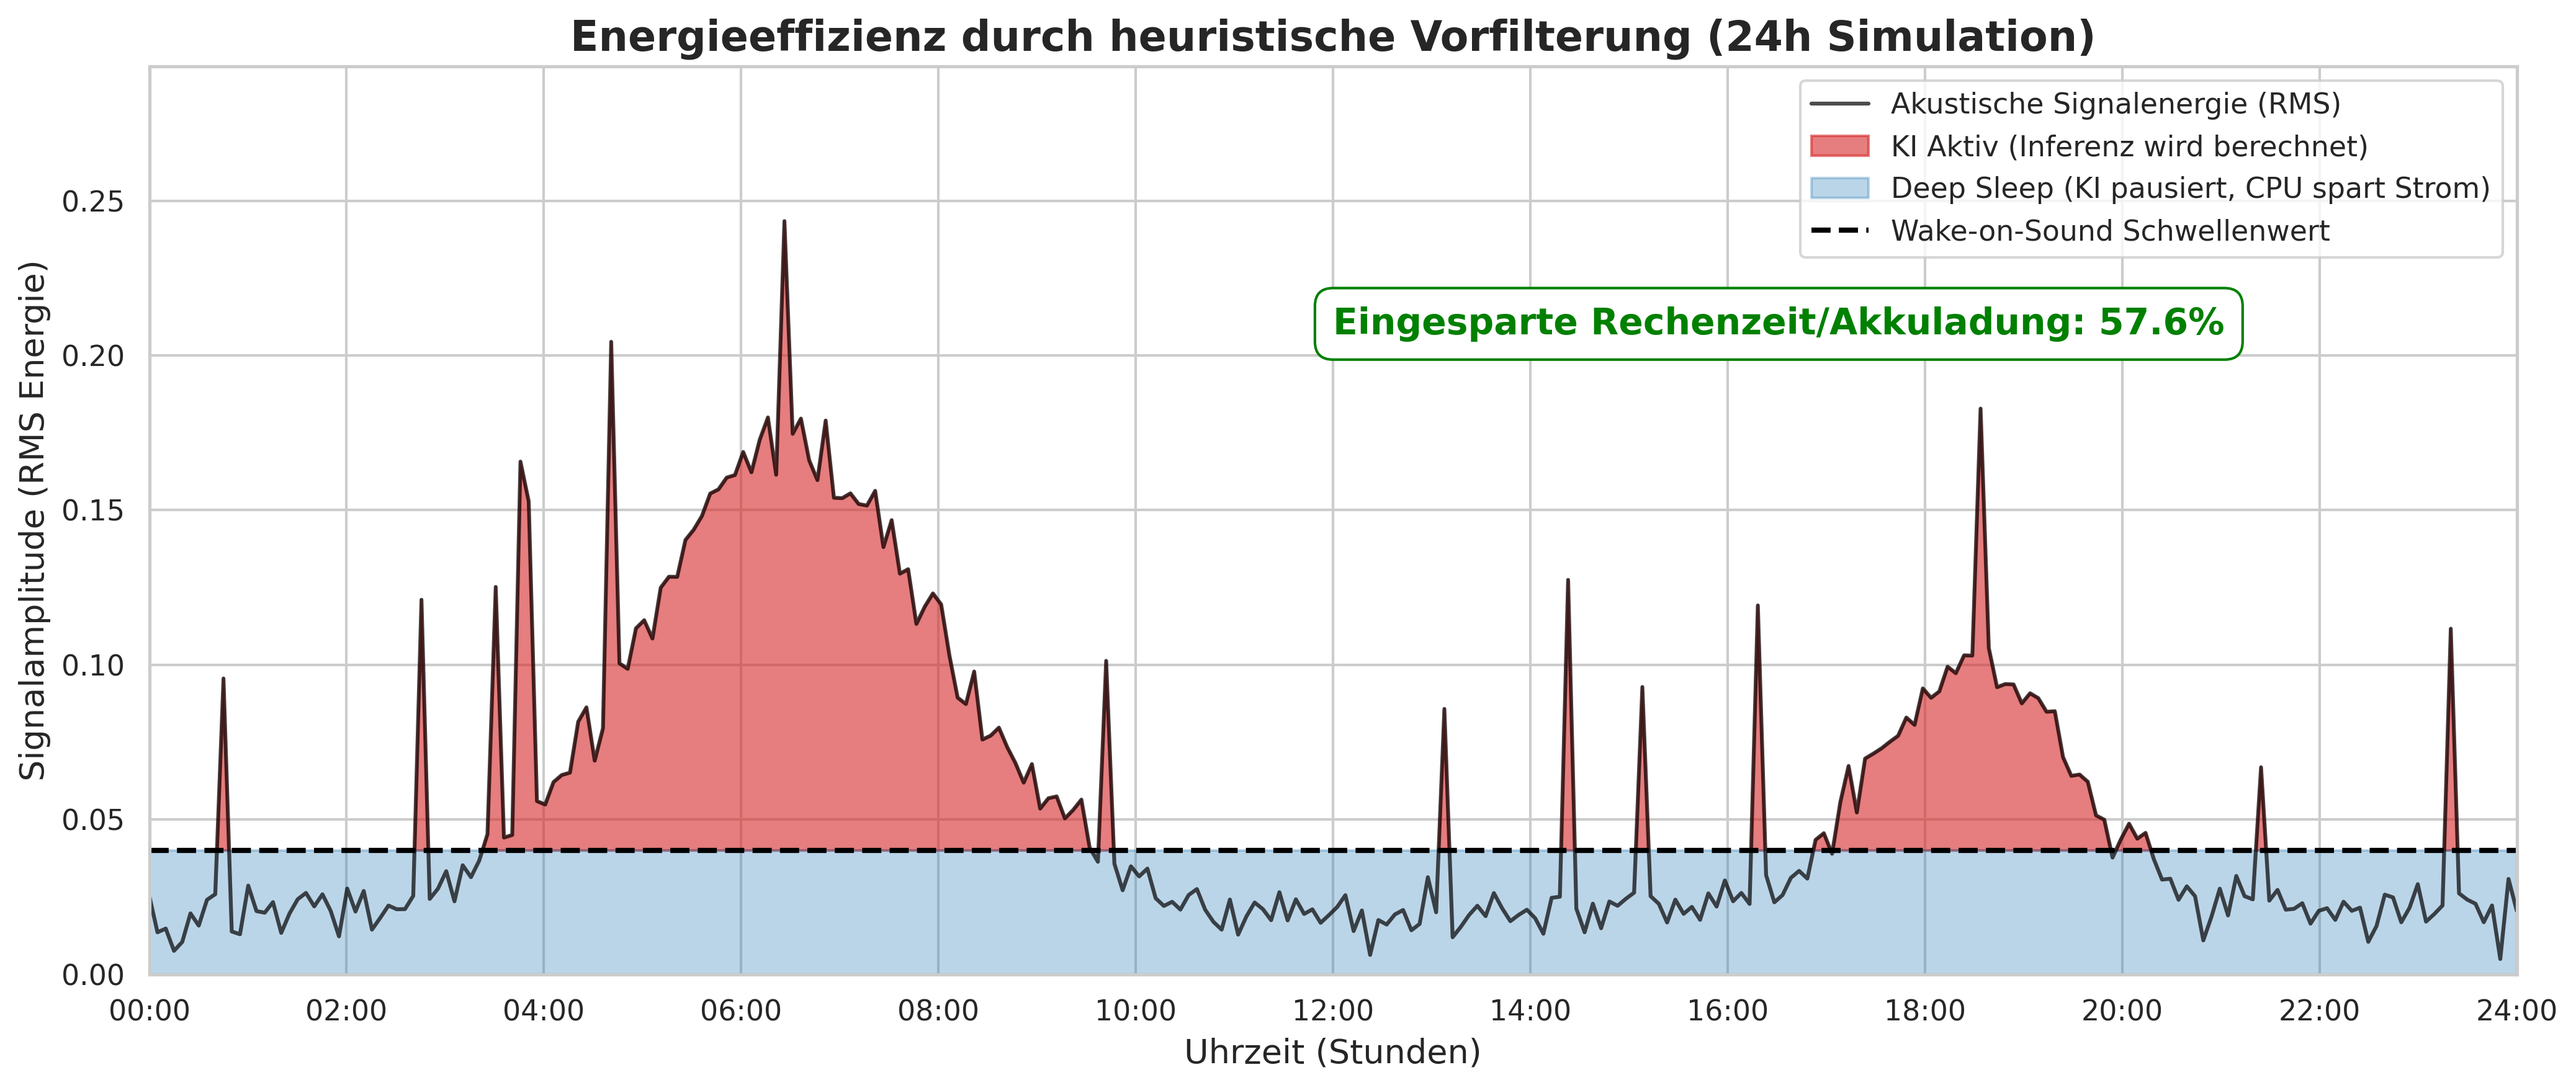
\includegraphics[width=\textwidth]{../visuals/experiments/wake_on_sound_energy.png}
    \caption{Simulierter Tagesablauf: Das rechenintensive CNN (rot) berechnet die Inferenz nur in lauten Phasen. In stillen Phasen (blau) schläft die KI, was den Akku massiv schont.}
    \label{fig:wakeonsound}
\end{figure}

\section{Fazit und Ausblick}
Wir konnten beweisen, dass die Kombination aus Open-Source-Daten, effizienten CNN-Architekturen und cleverem Post-Processing ein hochpräzises und ressourcenschonendes Edge-KI-System ermöglicht. Unser \enquote{Piepmatz Polizei}-Sensor ist in der Lage, autonom europäische Vogelpopulationen zu erfassen.

Der nächste entscheidende Schritt ist die wissenschaftliche Feldevaluation. In Kooperation mit Hobby-Ornithologen planen wir, unsere Prototypen zu im Wald zu testen. Dies wird die abschließende Bestätigung liefern, wie zuverlässig das System wirklich ist.

% --- Literaturverzeichnis ---
\newpage
\renewcommand\refname{Quellen- und Literaturverzeichnis}
\begin{thebibliography}{9}

\bibitem{kahl2021}
Kahl, S., et al. (2021).
\textit{BirdNET: A deep learning solution for avian diversity monitoring.}
Ecological Informatics.

\bibitem{tan2019}
Tan, M., \& Le, Q. V. (2019).
\textit{EfficientNet: Rethinking Model Scaling for Convolutional Neural Networks.}
arXiv preprint arXiv:1905.11946.

\bibitem{specaugment}
Park, D. S., et al. (2019).
\textit{SpecAugment: A Simple Data Augmentation Method for Automatic Speech Recognition.}
Proc. Interspeech 2019.

\bibitem{xenocanto}
Xeno-Canto Foundation.
\textit{Xeno-canto: Sharing bird sounds from around the world.}
\url{https://www.xeno-canto.org/}

\bibitem{pytorch}
Paszke, A., et al. (2019).
\textit{PyTorch: An Imperative Style, High-Performance Deep Learning Library.}
Advances in Neural Information Processing Systems.

\bibitem{onnx}
Bai, J., et al. (2019).
\textit{ONNX: Open Neural Network Exchange.}
\url{https://onnx.ai/}

\bibitem{eea2020}
European Environment Agency (2020).
\textit{State of nature in the EU: Results from reporting under the nature directives 2013-2018.}
EEA Report No 10/2020.

\end{thebibliography}

% --- Unterstützungsleistungen ---
\newpage
\section*{Unterstützungsleistungen}
Daten und Programme der Open-Source-Community haben die Umsetzung unseres Projekts sehr erleichtert. Insbesondere die Audiodaten von Xeno-Canto waren essenziell. Für die Programmierung haben wir Bibliotheken wie PyTorch, Librosa und Audiomentations genutzt. Ein Dank geht an unsere Informatik-Lehrer für das Feedback zwischendurch sowie an David May für die Gestaltung des Titelbildes.

Besonderer Dank gilt unseren JuFo-Betreuern für die anhaltende Unterstützung.

\end{document}
